\documentclass[11pt,a4paper]{article}
\usepackage{od}
\usepackage[utf8]{inputenc}
\usepackage[main=german,russian]{babel}

\title{Das System von Handlungs-Natur-Verhältnissen} 

\author{Piotr Georgievich Shchedrovitsky}
\date{10.11.2012}

\begin{document}
\maketitle
\begin{quote}
  Übersetzt von Hans-Gert Gräbe, Leipzig.
  
  Quelle: \foreignlanguage{russian}{Пётр Щедровицкий. Деятельностно-природная
    система. Журнал «Человек и природа». — М., «Знание», 1987, № 12,
    с. 12–63}.  Digitale Publikation unter
  \url{https://gtmarket.ru/laboratory/expertize/5412}
\end{quote}

\tableofcontents
\clearpage

\section*{Anmerkungen zur Übersetzung}

Die Schwierigkeit einer Übersetzung liegt in der genauen Wahl der übersetzten
Begriffe, was bei einer philosophischen Arbeit doppelt problematisch ist.
Auch in dieser Arbeit gibt es eine Reihe von russischen Begriffen, die keine
oder mehrdeutige deutsche Entsprechungen haben. Die wichtigsten Differenzen
sind hier aufgelistet:
\begin{itemize}
\item Der zentrale Begriff \foreignlanguage{russian}{деятельность} der Arbeit
  hat mehrere deutsche Pendants und ist als \emph{Tätigsein}, \emph{Tätigkeit}
  oder \emph{Handeln} übersetzt. Damit verbunden ist allerdings auch eine
  semantische Aufspaltung, die vom Autor in dieser Form möglicherweise nicht
  intendiert ist oder sogar kontraproduktiv in dem Sinne, dass jener Begriff
  in der Theorie eine Klammer um Kontexte bildet, die der Autor bewusst
  \emph{nicht} separieren möchte. Das von diesem Substantiv abgeleitete
  Adjektiv \foreignlanguage{russian}{деятельностно}, insbesondere in der
  zentralen Konstruktion \foreignlanguage{russian}{деятельностно-природная
    система}, hat überhaupt kein deutsches Pendant und wurde meist mit
  \emph{handelnd} übersetzt, die zentrale Konstruktion substantivierend als
  \emph{Handlungs-Natur-System}.  Auch das trifft die Intentionen des Autors
  nicht präzise.
\item Umgekehrt ist es mit dem Begriff \emph{Natur}, der im Russischen als
  \foreignlanguage{russian}{природа}, aber auch als Adjektiv
  \foreignlanguage{russian}{натурально} auftaucht mit deutlich differierender
  Semantik, so dass sich die Wortkonstruktion
  \foreignlanguage{russian}{натуральная природа} nur sehr ungenau als
  \emph{natürliche Natur} übertragen lässt.  In der Arbeit wird überwiegend
  das Wort \foreignlanguage{russian}{природа} verwendet, oft allerdings in
  Quotes, um eine gewisse Distanzierung des Autors von der gewöhnlichen
  Verwendung dieses Begriffs zu verdeutlichen. Die Quotes sind in der
  Übersetzung erhalten.

  Als dritter Begriff ist hier noch das Adjektiv
  \foreignlanguage{russian}{естественно} zu nennen, das im Kontext
  \foreignlanguage{russian}{естественно-научный} als naturwissenschaftlich und
  im Kontext \foreignlanguage{russian}{естественно-истори\-ческий} als
  natürlich-historisch übersetzt wurde.
\item Schließlich wird immer wieder der Begriff
  \foreignlanguage{russian}{объект} gebraucht, der im Deutschen wohl besser
  als \emph{Gegenstand} übersetzt wird, hier aber weitgehend als \emph{Objekt}
  übertragen wurde.
\end{itemize}

\section*{Zum Autor des Aufsatzes}

Piotr Georgievich Shchedrovitsky ist ein russischer Philosoph, Methodologe,
Gründer und Leiter der Schule für Kulturpolitik. Er absolvierte die Fakultät
für Pädagogik und Psychologie am Moskauer Staatlichen Pädagogischen Institut,
arbeitete an Fragen der Psychologie, der Managementmethodik, der Organisation
angewandter komplexer Forschung in verschiedenen Bereichen (Pädagogik,
Management, Rohstoff\-förderung) sowie auf dem Gebiet der Umweltbildung und
der Ausarbeitung von Umweltprogrammen auf der Grundlage methodischer Forschung
Forschungen.  Er hat dazu beigetragen, dass Begriffe wie „Kulturpolitik“,
„Russische Welt“, „Humanity-Technologien“ (zusammen mit E. Ostrovsky),
"geoökonomisches Gleichgewicht“ (zusammen mit V. Knyaginin),
„Anthropostrukturen“ und „Anthropoströme“ (zusammen mit S.  Gradirovsky) in
moderne Diskussionen Eingang gefunden haben. Er entwickelte Vorstellungen von
Framing-Techniken des Denkens und den ressourcenbasierten Ansatz konsequent
weiter. Er hat eine Reihe von Politikern, Parteien und staatlichen
Institutionen beraten.  Er war an der Erstellung von Entwicklungsstrategien
für eine Reihe russischer Regionen beteiligt.  Der hier vorgestellte Text
wurde erstmals 1987 veröffentlicht.

\section{Einleitung}

Die Situation, die sich im letzten Viertel des zwanzigsten Jahrhunderts in
Gebieten und Handlungsbereichen herausgebildet hat, in denen das Material der
Natur für menschliche Bedürfnisse erfasst und ausgenutzt wird, zwingt
Ideologen und Theoretiker, Organisatoren und Ingenieure, den sich in
Jahrhunderten herausgebildeten Korpus theoretischer und praktisch-methodischer
Ansätze zu einem großen Teil zu überdenken und zu revidieren: Technik und
Wissenschaft, Engineering und Lebensstile -- alle steht unter ökologischem
Zweifel. Viele gewohnte Handlungs- und Denkweisen müssen heute verworfen
werden.  Der produktive und konsumtive Enthusiasmus des zivilisierten Menschen
muss begrenzt werden. Die gewohnte Strategie des extensiven Wachstums
kollidiert mit einem ökologisch orientierten gesellschaftlichen Bewusstsein.

Was aber wird eigentlich die bestehenden Prinzipien der Organisation und
Leitung der sozialen Produktion ersetzen? Was sind die Perspektiven der
Entwicklung des Komplexes der Projeksteuerung und der Energetik? Was sind die
perspektivischen Linien der Entfaltung einer regionale ökologischen Politik?
Wie muss das Ingenieursdenken beschaffen sein, das abfallfreie und ökologische
Technologien schafft?

Es ist klar, dass es auf diese Fragen keine eindeutigen und vollständigen
Antworten gibt.  Gleichzeitig verstehen wir, dass die richtige
\emph{Formulierung der Frage} bereits die halbe Antwort ist.  Es ist
wichtiger, die Problemsituation zu skizzieren als eine bis zur letzten
Nachkommastelle korrekte Antwort auf eine Frage zu geben, die grundlegend
falsch gestellt ist. Um jedoch ein Gefühl für die tief\-liegenden Probleme zu
bekommen und die Hauptfragen herauszuarbeiten, sind \emph{neue Konzepte und
  Vorstellungen} erforderlich, auf die sich das Denken im Prozess der
Problematisierung, der Suche nach neuen Ansätzen und neuen Lösungen stützen
kann.  Ehe die einen oder anderen Projekte vorgeschlagen werden, muss ein
angemessener konzeptioneller Apparat gebildet werden, jene Sprache, in der
ökologische Programme und ökologische Aspekte der Entwicklung von sozialen
Systemen besprochen werden können.

Um die Problematik zu öffnen und die notwendigen Vorstellungen in der
notwendigen Weise zu umreißen, muss man sich der vorhandenen soziokulturellen
Situation zuwenden, müssen die Tendenzen der Änderung von Handlungsbereichen
herausarbeiten, die sich herausgebildet haben und das Gesicht der sozialer
Systeme prägen, muss die Grenzen der Situation selbst als problematische
ökologische Situation abstecken.

Dabei beginnen wir unsere Analyse mit konkreten Handlungsbereichen und
-feldern, betrachten private und lokale Schwierigkeiten und Paradoxien im
weiteren Sinne und ordnen sie ein als Manifestation allgemeiner Tendenzen des
Funktionierens und der Entwicklung von natürlich-technischen Systemen und
Systemen eines Handlungs-Natur-Verhältnisses.

\section{Extraktive Technologien: Bedingungen, Lage der Dinge, Situation}

Wenden wir uns den Erfahrungen des Managements in der Rohstoff\-industrie zu.
Der Verzicht auf primitive Zugänge und Technologien, die schnelle Effekte für
genügend einfache, oberflächennahe Lagerstätten versprechen, die Notwendigkeit
der Koordinierung verschiedener Infrastrukturen innerhalb der
Rohstoff\-industrie unter Hinzunahme breiterer wirtschaftlicher Mechanismen --
all das rückt heute Aufgaben von Organisation, Leitung und Steuerung im
weitesten Sinne in den Vordergrund. Die fallende Abbauergiebigkeit, zunehmende
Schwierigkeiten der geologischen und bergbaulichen Bedingungen der Gewinnung
von Bodenschätzen bleiben nicht ohne Auswirkungen auf die Vergrößerung der
organisatorischen Strukturen in der Rohstoff\-industrie; die Kompliziertheit
der Systeme spiegelt sich direkt im Charakter der Organisations- und
Managementarbeit wider. Bisher hat diese Änderung jedoch auf die extensiven
Parameter ausgewirkt -- die Frage der Qualität der Organisations- und
Managementarbeit wird nicht direkt gestellt und zieht keine Aufmerksamkeit auf
sich.  Aus unserer Sicht ist es heute notwendig, nicht nur den Stil, sondern
auch den gesamten Organisations- und Managementansatz in der
Rohstoff\-industrie grundlegend zu ändern.

Als Beispiel können wir uns auf die Situation innerhalb der Öl- und
Gasindustrie konzentrieren. Die erste Frage, die man sich stellen muss, wenn
man eine Analyse der Organisation- und Managementstrukturen dieser Sphäre
beginnen will, ist, welche Prozesse sind Führungspro\-zesse und gleichzeitig,
in welchem Rahmen muss das Objekt und der Gegenstand der Managementprozesse
beschrieben werden?  Etwa ist die Frage zu klären, ob die Förderung von Öl und
Gas ein produktiver oder ... ein Transportprozess ist.

Diese Frage ist grundlegend: Methoden und Formen des Managements in den beiden
Fällen unterscheiden sich grundlegend voneinander. Wenn wir davon ausgehen,
dass die Förderung von Öl und Gas ein Produktionsprozess ist, dann ist es
natürlich zu fragen, was produziert wird und was das Produkt dieser Produktion
ist. Auf diese Frage kann schon nicht mehr geantwortet werden: Öl und Gas. Öl
oder Gas selbst sind kein Produkt der Produktion; sie sind als Halbzeug oder
Primärrohstoff für einen Produktionsprozess zu betrachten, der über die
Extraktion hinausgeht.

Mit anderen Worten: Die Gewinnung oder Förderung von Öl und Gas selbst ist
kein Produk\-tions\-prozess. Außerdem, je nachdem, in welche größeren
organisatorischen und wirtschaftlichen Strukturen der Extraktionsprozess
eingeschlossen ist, wird er verschiedene Funktionen und verschiedene
organisatorische Belastungen haben. Wenn das geförderte Öl durch Pipelines ins
Ausland geschickt wird, dann ist die Förderung ein Teil eines Transportsystems
oder ein Teil des Außenhandels. Wird das geförderte Öl hingegen zu anderen
Produkten verarbeitet, wird die Förderung zu einem Teil des Transportsystems
oder zu einem Fragment des Außenhandels.  Wird es hingegen zu anderen
Produkten verarbeitet, so wird die Extraktion zu einem Teil eines
Produktionsprozesses.

Diese elementare Grammatik des Managements bewegt jedoch die Organisatoren in
der Roh\-stoff\-industrie in keiner Weise. Ohne über die Folgen und
Perspektiven ihrer Wahl der einen oder anderen Organisationsstrategie
nachzudenken, setzen sie naiv voraus, dass die Förderung von Öl und Gas selbst
ein eigenständiger Produktionsprozess ist, und verwenden alle sekundären
Methoden der organisatorischen und wirtschaftliche Analysen, welche die
Effektivität und die „wirtschaftlichen“ Vorteile des gewählten Ansatzes zeigen
sollen.

Nur ein radikaler Bruch mit bestehenden Stereotypen und druch äußere
Einwirkung bewirken, dass die Organisatoren beginnen, die Situation zu
reflektieren. Der Verfall der Ölpreise auf dem Weltmarkt zeigt zum ersten Mal,
dass der Verkauf weder effizient noch profitabel ist. Es stimmt, dass bereits
im 13. Jahrhundert die einfache merkantilistische Weisheit formuliert wurde,
dass es profitabler ist, verarbeitete Waren zu verkaufen als der Verkauf von
Rohstoffen. Aber die Festigkeit etablierter Verwaltungsprinzipien ist stärker
als merkantilistische Weisheit. Es ist nun notwendig, die übliche Strategie
aufzugeben und eine wirklich organisatorische Managementaufgabe zu lösen: was
und wie soll produziert werden?

Übrigens ist diese Frage alles andere als trivial. Alle Nebenprodukte sind ein
Moment und Fragment innerhalb des Brennstoff-Energie-Komplexes und damit ein
Moment des Systems der gesellschaftlichen Reproduktion. Mit anderen Worten,
wenn wir Benzin und Heizöl produzieren, produzieren wir es natürlich, aber
Sinn erhält diese Produktion erst im Rahmen eines größeren Systems -- wiederum
eine einfache Systemweisheit.

Aber dann, wenn man mit der Organisations- und Managementanalyse fortfährt,
ist es natür\-lich zu fragen: Welches Gewicht und welchen Status hat die
Förerung von Öl und Gas im Rahmen des Brennstoff-Energie-Komplexes?  Wenn die
Frage so gestellt wird, müsste der Organisator anfangen nachzudenken. Er würde
ein Stück Papier und einen Stift nehmen und zunächst einmal alles zählen, was
den Brennstoff-Energie-Komplex des Landes ausmacht.  Kernkraft, Wasserkraft,
Kohle, Öl und Gas, Solar- und Wasserkraftwerke, neue Motoren und neue
Autodesigns, neue Arten von Rahmen und Fensterglas ... Mit einer solch
einfachen Aufzählung kann eine Reihe von komplexen Forschungs- und
Entwicklungsprogrammen initiiert werden, die auf eine Verringerung des Gewicht
der Förderung und des Verbrauchs von Öl und Gas innerhalb des
Brennstoff-Energie-Komplexes gerichtet sind, um diesen wertvollsten Rohstoffe
aus den bestehenden Mechanismen der nicht-rationalen Nutzung herauszulösen und
in den Rahmen des chemisch-rohstoff\-lichen Komplexes zu verschieben.

Die gleiche einfache merkantilistische Weisheit zeigt, dass es wesentlich
effizienter ist, auf der Basis von Erdölprodukten Medikamente herzustellen als
Heizöl. Mit anderen Worten, man könnte die Extraktionstechnologie nicht in den
Rahmen der Reproduktion und brennstoff-energetischen Absicherung des
Wirtschaftsmechanismus einordnen, sondern in die Rahmen der Entwicklung und
Schaffung neuer Biotechnologien und Heilpräparate.

Wenn man anerkennt, dass die Rohstoff\-industrie heute ein sehr komplexes
organisatorisch-technischen System bildet, sind wir verpflichtet, die Frage
nach den optimalen organisatorischen \emph{Strategien und Prinzipien}, die
dieser Art von System adäquat sind, auf die Tagesordnung zu setzen. Wir müssen
uns von einer falschen Produktionsideologie verabschieden, nach der sich
herausstellt, dass das geförderte Öl (manchmal 12--15 Prozent der Vorräte, und
noch auf eine solche Weise, dass die verbleibenden 85 Prozent nie extrahiert
werden können) ein Produkt ist, der stoff\-liche Nachweis der Produktivität.
Wir müssen neue Programme auf\-legen -- sowohl in bei der Suche nach
alternativen Kraftstoffen (das macht jede Ölfirma im Ausland), als auch im
Bereich prinzipiell neuer Formen der Nutzung von Öl und Erdölprodukten.  Wir
sind heute mit der Notwendigkeit konfrontiert, die Frage neu zu prüfen und zu
lösen, was die prinzipiellen Managementstrategien in der Rohstoff\-industrie
sind.  Worauf kann sich der Organisator und Manager stützen, wenn er plötzlich
beschließt, sich von den „großväterlichen“ Zugängen zu den natürlichen
Möglichkeiten der Erde zu verabschieden?

Wir müssen verstehen, dass die Rohstoff\-industrie nicht nur ein komplexes
organisatorisch-technisches System ist. Es ist ein organisatorisch-technisches
System auf natürlichem Material. Mit anderen Worten: Die organisatorischen und
technischen Systeme in diesem Bereich \emph{„parasitieren“ auf natürlichem
  Material}, verbrauchen und verarbeiten dieses Material, wirken auf dieses
ein, indem sie jeweils relativ große Zonen und Areale des Territoriums
ausbeuten -- Länder, Wälder und Wasser.

Der Charakter solcher Art von Einwirkungen ist immer sehr schwer vorhersehbar
und gleichzeitig ist es organisatorisch sehr schwierig, echte Grenzen des
Systems zu ziehen, über dessen Management wir sprechen. Handlungsorientierte
und natürliche Momente „leben“ in verschiedenen Zeiten und folgen
verschiedenen Gesetzen, sie sind veschiedener Logik unterworfen, was bedeutet,
dass auch die Zugänge zu ihnen verschieden sein müssen. Indem diese oder jene
für einen gegebenen Handlungstyp führende, vorherrschende Art von
Naturmaterial verbraucht oder verarbeitet wird, wirken diese Systeme auf ein
größeres Areal, transformieren dessen Charakteristiken wesentlich und
verändern damit die Handlungsbedingungen anderer wirtschaftlicher
Infrastrukturen.

\section{Die ökologische Lage: erste Orientierungspunkte}

Bis vor kurzem hat sich im Managementbereich der Mythos von der
„Unerschöpf\-lichkeit“ der Ressourcen der Erde gehalten. Oftmals, wenn
ökologische Fragen mit wirtschaftlichen Entscheidungsträgern aller Ränge
erörtert wurden -- wie in der Rohstoff\-industrie, so auch in der Bauindustrie
-- hört man Selbstberuhigung: „Das Land ist groß“ ...  Es macht sich eine
jahrzehntelange Tradition von Haltungen und Überzeugungen in Bezug auf die
natürlichen und menschlichen Ressourcen bemerkbar, ein Führungsstil und die
Selbstdefinition eines „Managers auf zwei Jahre“ -- eines Managers auf Zeit.

In den letzten Jahrzehnten hat das Ausmaß des anthropogenen und technogenen
Einflusses auf die Umwelt soclhe Maßstäbe erreicht, dass der gesamte Planet
und das Leben selbst auf ihm gefährdet ist. Immer mehr Spezialisten, breitere
Gruppen der Öffentlichkeit diskutieren und analysieren die ökologische
Situation, wie sie sich in verschiedenen Bereichen, Handlungsfeldern und
geografischen Zonen entwickelt hat. Die Problematik der Ökologie ist auf der
Prioritätenliste nationaler Themen ganz nach oben gerückt. Alle sprechen über
Ökologie, die Umweltbewegung nimmt Fahrt auf, deren Vertreter beharren auf
einer grundlegenden Änderung der bestehenden technologischen und
organisatorischen Strategien und individueller Lösungen.

Allerdings weiß niemand wirklich, was das ist -- Ökologie, und was die
Prinzipien und Ansätze sind, auf die sich ein neues -- ökologisches -- System
des Wirtschaftens stützen soll.  Das erste, womit man unmittelbar konfrontiert
ist und worauf das ökologische Bewusstsein drängt, das ist der Fakt der
unberücksichtigten und unkontrollierbaren Folgen von technogenen Einwirkungen
auf die natürliche Umwelt.  Indem man es mit komplizierten Handlungssystemen
zu tun hat, die auf Naturmaterial parasitieren, befinden wir uns ständig in
der Situation des Auseinanderfallens, des „Zerreißens“ zwischen den
Handlungszielen und den tatsächlichen Folgen und Ergebnisse dieser Handlungen.
Das Fehlen einer adäquaten Vorstellung vom „Leben“ der Natur unter technogenen
Einwirkungen macht sich sofort bemerkbar, wenn wir über die Grenzen von
Prinzipien und Maßstäben der Einflussnahme auf die Natur, die sich über
Jahrhunderte bewährt haben, hinausgehen.

Die realen Folgen weichen stark von den Erwartungen und Prognosen ab, Folgen
von Sekundärmaßnahmen zur Kompensation der ursprünglichen Folgen weichen
wiederum von den Zielen ab, und... so weiter. Die Folgen nehmen einen
lawinenartigen unkontrollierbaren Charakter an, und wir leben faktisch in
einer Welt der „Nachbehandlungen“ unserer eigenen Züge, in einer künstlichen,
von uns erdachten und erschaffenen Welt. Ein Unglück kommt hinzu: auf den uns
umgebenden Erscheinungen und Kataklysmen kann niemand Schilder mit Hinweisen
und Preisen anbringen, wer, wann und wie diese Folgen hervorgerufen hat, für
die wir im Prinzip „zahlen“, und wie lange wir nch gezwungen  sind zu zahlen.  

Das Ausmaß dieser Erscheinungen ist wirklich katastrophal, wir haben es mit
einer breiten ökologische Situation zu tun, die viele Ideologen, Theoretiker
und gesellschaftlich Tätige vollkommen zu recht als Situation einer
ökologischen Krise bezeichnen und nicht mit apokalyptischen Prognosen sparen.

Es ist schwierig, auf die Fragen zu antworten: Wie können wir die Auswirkungen
unseres Handelns erfassen und kontrollieren, was müssen wir tun, um eine
ökologische Katastrophe abzuwenden, und woran muss ein Organisator denken, der
es mit dieser Art von heterogenen und heterarchisierten Systemen zu tun hat,
die sowohl Handlungs- als auch natürliche Komponenten umfassen?

Wo, in welchem Wissensgebiet können wir nach Antworten auf diese Fragen
suchen? Fakt ist, dass wir die ökologische Situation nicht ignorieren können.
Fakt ist auch, dass nicht bekannt ist, wie sie berücksichtigen. In den letzten
Jahren sprechen wir über \emph{rationale Naturnutzung}, über Strategien der
Ressourcenschonung, über rationale Territorialerschließung. Entfernt man
jedoch das Wort „rational“, dann bleibt im Großen und Ganzen das, was ist.
Natur wird weiter genutzt und Territorien werden weiter erschlossen. Es dreht
sich also alles, einfach gesagt, um diese noch unerreichbare Rationalität.
Und sie kann nirgendwo anders herkommen als aus dem Reich der Vernunft, durch
Ausdehnung der Vernünftigkeit auf das neue Feld der menschlichen sozialen
Tätigkeit, durch die Einführung und Etablierung rationaler Orientierungen
sowohl im Bereich des Bauwesens wie auch in der Rohstoff\-industrie.

V. Vernadsky schrieb über die „Noosphäre“ -- die Sphäre der Vernunft. Wir
sprechen über rationale Naturnutzung. Aber diese Rationalität muss sich noch
etablieren, muss konstruiert, in Gedanken geformt und dann umgesetzt werden --
zunächst in experimentellen Regionen, und dann auf der Ebene des Landes.  In
dieses Konzept der Rationalität müssen zweifellos Konstruktionsprinzipien
ökologischer Systeme und ökologischer Technologien eingehen, Schemata der
Rehabilitation und Wiederherstellung von Naturarealen, Prinzipien
wettbewerbsbasierter und alternativer Projektierung technischer Systeme und
vieles mehr.

Gleichzeitig muss die Rationalität mit irgendetwas beginnen. Und natürlich
sollte sie mit vorhandenen Erfahrungen in den Bereichen der Ausarbeitung,
Projektierung, Exploration, Konstruktion, Gewinnung, Verarbeitung, Lagerung
beginnen, mit dem reichen Erfahrungsschatz organisatorischen, wirtschaftlichen
und produktiven Handelns. Aber falls sich der Organisator entscheidet, sich
den Erfahrungen des Handelns zuzuwenden, wird er sich vor allem überzeugen,
dass es einfach keine solchen Erfahrung gibt, überhaupt keine! Sie als Leser
können natürlich fragen: Wieso das -- keine Erfahrungen? Man kann auch Sie
fragen: woher sollen sie kommen?  Gibt es eine Dienststelle für die Analyse
und Verallgemeinerung von Erfahrungen, vor allem natürlich von negativen?
Gibt es etwa eine Institution, die Informationen, Analysen und Kritiken von
Erfahrungen mit Havarien, erfolglosen Konstruktionen, vorzeitige Erschöpfung
und Still\-legung von Lagerstätten sammelt? Gibt es etwa irgendeine Instanz,
die für die Verallgemeinerung und Verbreitung dieser Misserfolgs-Erfahrungen
verantwortlich ist... damit andere nicht dieselben Fehler machen? In Ordnung,
das sind negative Erfahrung. Aber auch positive Erfahrungen, erfolgreiche
Lösungen und Entdeckungen werden von niemandem analysiert, es werden keine
Schemata der Organisation von Handlungen und Produkten herausgearbeitet, sie
werden nicht mit entsprechenden Modifikationen in anderen Regionen und
Bereichen umgesetzt. Kann es sein, dass es positive Erfahrung einfach nicht
gibt, sondern nur negative?

Und so werden Fehler und falsche Entscheidungen über Jahrzehnte ohne
Veränderung wiederholt und reproduziert, mit außergewöhnlicher Konstanz und
Zielstrebigkeit.  Lagerstätten verwandeln sich überall von Öl fördernden zu
„Wasser fördernden“, und die Erfahrung, Öl mit Wasser zu verdrängen, wird
angewendet und wird auch in Zukunft weiter angewendet werden!  Es werden
Schlammspeicher gebaut, auch weiterhin in der gleichen bewährten Art und
Weise, obwohl alle gebauten undicht sind, auslaufen und damit viele Tausende
Hektar Land für immer unbrauchbar für eine weitere Nutzung machen!  Es werden
riesige Gasverarbeitungskomplexe geplant, gebaut und werden auch weiter
gebaut, obwohl deren Ineffizienz und Irrationalität längst bewiesen ist!

„Wir haben es so gemacht und wir werden so machen“. Dies ist das Prinzip, das
sich jeder Erfahrung widersetzt, diese verneint und ablehnt.

Man kann sich natürlich fragen, warum werden eigentlich Erfahrungen --
positive wie negative -- nicht genutzt und nicht berücksichtigt? Man kann sich
beschweren: Wenn man...  Aber dabei muss man gut verstehen, dass die
verbreitete Haltung zu Erfahrungen aus Ausarbeitungen und Planungen eine
gesetzmäßige und natürliche Sache ist.  Anders: im bestehenden System der
Arbeitsorganisation kann es anders nicht sein. Erfahrung wird nur in solchen
Systemen benötigt, in denen eine bewusste und zielgerichtete Suche nach neuen
Methoden und Ansätzen zur Problemlösung stattfindet. Erfahrung wird dort
benötigt, wo Innovation eine Regel der normalen Organisation von Handeln ist.
In allen anderen Fällen sind Erfahrungen (positive wie auch negative) nicht
nur unnötig, sondern auch direkt schädlich.

Auswahl, Analyse, Kritik, Fixierung in verallgemeinerten Formen, Verbreitung
und Einfüh\-rung von neuen oder überhaupt irgendwelchen Erfahrungen ist ein
besonderes organisatorisch-steuerndes Handeln, das auf Veränderung,
Transformation, und letztendlich auf die ständige \emph{Entwicklung}
bestehender Systeme und Handlungs-Strukturen gerichtet ist. Wenn es eine
solche Einstellung nicht gibt, wenn die verschiedenen Dienste und
Infrastrukturen sich nicht entwickeln und ihr Handeln ändern wollen, dann wird
jede Erfahrung natürlich und rigoros vom System zugunsten der gewohnten
Arbeitsformen abgelehnt und im Falle von administrativem Zwang in solchen
Formen verwendet und umgesetzt, dass diese „neue Erfahrung“ den bewährten
Prototypen extrem ähnlich sein wird.

Und es geht hier nicht darum, dass die Erfahrung nicht beschrieben und
analysiert würde. Der Punkt ist, niemand braucht diese Erfahrung; keine
einzige Institution ist an solchen Erfahrungen interessiert, und damit an der
Abgrenzung und Fixierung einer Zone notwendiger Umformungen und der
Entwicklung eigener Aktivitäten. Wir haben es so getan und werden es auch
weiterhin so tun! Und umgekehrt: Solange die bestehenden Systeme der
Rohstoff\-industrie und des Bauwesens, des Brennstoff-Energie-Komplexes und
des Verkehrswesens nicht ganz und vollständig auf die permanente Umgestaltung
aller Denk- und Handlungsstrukturen in ihrer Sphäre eingestellt sind -- bis
dahin wird niemand neue Erfahrungen brauchen und wir werden die Fehler und
Paradoxien der vergangenen Jahrzehnte reproduzieren und... die ökologische
Situation verschlimmern.

Aber was wäre, wenn...

Wenn diese Art Strategie der permanenten Veränderung oder Entwicklung
angenommen würde und verschiedene Arten von Institutionen auf diese
Erfahrungen zurückgreifen würden, würden sie wiederum enttäuscht. Denn --
aufgrund der historischen Lage der Dinge und der vollständigen
Niemand-braucht-sie-Lage der gesuchten Erfahrungen -- weiß heute niemand, wo
diese Erfahrungen zu suchen und welche Typen von Arbeiten auszuführen sind, um
dennoch an diese heranzukommen. Keiner weiß, in welcher Form die Erfahrung des
Denkens und Handelns in Situationen erfasst werden kann und muss, die wir als
ökologische ansehen.  Wie kann sie von einer Situation auf eine andere
übertragen und übersetzt werden? Wie soll sie schließlich verbreitet und
umgesetzt werden?  Erfahrung als „Ding“ der geistigen Welt, erfordert
besondere Arten der Handhabung. Um Erfahrungen aus der Förderung von Öl und
Gas zu ziehen, bedarf es einer völlig anderen Organisation von Handeln selbst:
insbesondere Normierung, Etalonisierung, Standardisierung, Manufakturisierung
des Handelns. Also letztendlich wieder -- Rationalisierung.

Es scheint, dass wir in einen Teufelskreis geraten. Die Voraussetzung für die
Rationalisierung von Denkens und Handeln in den Rahmen einer ökologischen
Situation ist die Analyse und Verallgemeinerung von Erfahrung, und die
Bedingung für das Herausarbeiten und Fixieren von Erfahrung ist die
Rationalisierung des Denkens und Handelns.

\section{Verallgemeinerung der Erfahrung und die Probleme der Erforschung
  techno-natürlicher Objekte} 

In Handlungssystemen funktionieren die physikalistischen Modelle von „Anfang“
und „Ende“ nicht.  Handeln und Denken haben viele Anfänge; die Kunst des
Organisators besteht darin, die fortschreitende und vernetzte Entfaltung einer
Vielzahl von Prozessen zu sehen und zu kontrollieren. Die Bildung eines
„Erfahrungsschatzes“ ist, dem Wesen nach, nur ein und wahrscheinlich nicht der
wichtigste Kanal der Rationalisierung und Steuerung. Jede Lagerstätte ist
\emph{einzigartig}. In dieser Hinsicht ist eine direkte Übertragung der
bestehenden Schemata der Organisation von Handeln auf eine neue Situation
nicht möglich, wie auch immer die Erfahrung der vorausgegangenen Entwicklungen
organisiert ist. Um vorhandene Erfahrung in die Konstruktion des Neuen und die
Gestaltung der Zukunft einzubringen, muss diese noch besonders präpariert
werden.  Erfahrung muss \emph{typologisch} dargestellt werden.

In der Tat sind Typologie und die typologische Methode jene prinzipiellen
logisch-methodolo\-gischen Formen, die eine Systematisierung un
Verallgemeinerung der Erfahrung aus einzelnen Ausarbeitungen gestatten, um
diese Erfahrungen dann von einer auf eine andere Situation zu übertragen.
Allerdings können die Typologien selbst und die typologischen Methoden
dahinter verschieden sein. Das können phänomenale Typologien sein, die sich
auf eine Systematisierung und Verdichtung von Erfahrungen und Wissen über
reale Lagerstätten stützen, auf technisch-technologische Aspekte der
Ausarbeitungen und die ökologischen Folgen. Aber solche Typologien geben uns
wenig bei der Gestaltung von Neuem.

Die Arbeit wird anders aufgebaut, wenn wir uns mit Idealtypen beschäftigen,
und damit mit einer konstruktiven Typologie, die sich auf eine theoretischer,
denkerische Basis stützt -- auf die Vernunftsphäre. Eine konstruktive
Typologie führt uns direkt zum Design und zur Programmierung von Handlungen;
sie bereitet in gewisser Weise die Zukunft vor. Aber dann muss als Grundlage
dieser typologischen Arbeit nicht so sehr die Analyse erfolgreicher (oder
erfolgloser) Erfahrungen dienen, nicht so sehr die Beschreibung und Kritik
bestehender Präzedenzfälle und Prototypen, sondern vielmehr eine spezielle
Denkarbeit, die breite \emph{Untersuchung} von Handeln und Handlungssystemen,
die sich auf der Basis von Naturmaterial vollziehen.

Zugleich stößt die Organisation solcher Art von Forschung auf ernste
methodologische Schwierigkeiten. Um Forschung aufzubauen, benötigt man ein
System von Modellen und ontologischen Bildern -- jene idealen Objekte, an
denen sich die Forschungsarbeit selbst entfalten wird. Aber jne idealen
Objekte gibt es in den heute verbreiteten theoretischen und ideologischen
Konzepten nicht.

Es gibt natürlich unmittelbare Objekte oder -- genauer gesagt -- Objekte der
organisatorisch-praktischen Operation und Beeinflussung. Aber leider sind das
nicht die Objekte, die für die Forschung benötigt werden. Mit solchen
phänomenal gegebenen Objekten kann der Forscher einfach nichts anfangen.

Eine einzelne Lagerstätte, Ablagerung, Verwerfung, ein Naturraum kann nicht
das Objekt von Forschung sein. Der Übergang zu Engineering und
ingenieur-technischen Konstruktionen im Bereich der Entwicklung von Maschinen
und Mechanismen wurde erst möglich, nachdem ein System idealer Objekte der
„Mechanik“ und die entsprechende Theorie naturwissenschaftlichen Typs
ausgearbeitet waren. Kann jedoch eine \emph{Wissenschaft vom Galileischen Typ}
ihre Anwendung im Bereich der Ökologie finden? Geht man von der These aus,
dass in der extraktiven Industrie kein System von idealen Objekten
ausgearbeitet und konstruiert wurde, muss man noch fragen: können uns hier die
Muster und Prototypen der Naturwissenschaften helfen?  Welche Art von Typen
und Geräte sollten die idealen Objekte sein, auf deren Basis wir die für uns
so notwendigen Forschungen und Ausarbetungen aufbauen können?

Wir wollen mit einer Antwort nicht voreilig sein. Die traditionelle Geologie
hat im Kern eine ganze Reihe von ideal-phänomenalen „Objekten“ geformt, an
denen sich heute Wissenschaftler und Praktiker in den extraktiven Zweigen
überwiegend orientieren.  Die traditionelle Geographie erhebt den Anspruch,
die führende Disziplin im Komplex der Geowissenschaften zu werden. Allerdings
taugen, aus unserer Sicht, diese „Objekte“ einer traditionell
aktualistischen, historischen oder naturwissenschaftlichen Geologie und
Wirtschaftsgeographie nicht als Objekte einer an Aufgaben des Managements
ökologischer Situationen orientierten Forschung.

Schließlich hat es der Organisator in diesem Bereich mit einer komplexen --
heterogenen und heterarchischen - Gesamtheit zu tun, die aus Handlungs- und
Naturkomponenten besteht.  Die Handlungs-Fragmente „leben“ nach den einen
Gesetzen, während die Natur-Fragmente anderen Gesetzen folgen, die sich in der
überwältigenden Mehrheit der Fälle grundlegend von den Handlungs-Gesetzen
unterscheiden.  Daraus folgt, dass, wenn die Ganzheit, mit welcher es der
Operator zu tun hat, heterogen ist, macht es keinen Sinn, es in zwei Teile zu
zerlegen und zu stratifizieren und dann jedes Teilsystem in seiner eigenen
Sprache zu beschreiben. Jenes geologische Objekt, das in einer rein
geologischen Analyse -- ohne jede Beziehung zur technisch-technologischen
Komponente -- isoliert und erhalten wurde, wird völlig anders „leben“ und sich
verhalten als „das gleiche“ (aus einer systemischen Sicht aber in keiner Weise
das gleiche, sondern etwas prinzipiell anderes!) Objekt, das in eine neue
Ganzheit eingeschlossen ist.  Und umgekehrt wird sich die tätigkeitsbezogene,
technische Komponente außerhalb und getrennt von ihren Verbindungen zur
natürlichen Umgebung vollkommen anders verhalten, als „dieselbe“ Komponente
(im Kern -- überhaupt nicht sie!) im Rahmen dieser Ganzheit.

Mit anderen Worten, egal, wie sehr man die Handlungs- und Natur-Komponenten
auch je einzeln untersucht, wird es praktisch unmöglich sein, etwas über das
Handlungs-Natur-System als Ganzes zu sagen. Für die Forschung ist diese
Schlussfolgerung radikal. Um eine an Managementpraxen orientierte
wissenschaftliche Forschung aufzubauen, ist es -- grob gesagt -- notwendig,
alle traditionellen geologischen und geografischen, natürlichen Objekte zu
verwerfen und eine \emph{neue Realität des Denkens} zu konstruieren: eine Welt
von techno-natürlichen und natürlich-technischen Objekten verschiedener
Komplexitätsstufen, eine spezielle -- typologisch und systematisch
organisierte -- \emph{Technik-Natur-Ontologie}. Und die Objekte, die diese
neue Welt bevölkern, werden sich so stark von den traditionellen Objekten der
Geologie unterscheiden wie -- nach Spinozas bildlichem Ausdruck -- das
Sternbild des Hundes von einem Hund als bellendem Tier.

Und bis dahin, bis durch besondere konstruktive und gedankliche Arbeit eine
solche Welt gebaut ist, ist es leichtsinnig, von effektiven
Managementstrategien in der extraktiven Industrie, von rationeller Nutzung der
Natur und von der Entwicklung von Gebieten, von ressourcensparenden
Technologien und sogar von der Analyse und Verallgemeinerung von Erfahrungen
aus vorhandenen Ausarbeitungen und Lösungen unter Berücksichtigung der
ökologischen Situation zu sprechen.

Geht es nur um Begriffe und um neue ideale Objekte? -- wird sich der
aufmerksame Leser fragen. In der Tat ist diese Frage durchaus berechtigt.
Allerdings sind die Begriffe, von denen von Anfang die Rede ist, nach den
Bedingungen der Argumentation, beschränkt auf die Praxis des Managements
ökologischer Situationen; die Konstruktion eines Begriffs ist nicht so sehr
eine Forschungs- als vielmehr eine Projektaufgabe. Wir brauchen Begriffe der
ökologischen Situation und Modellen techno-natürlicher Systeme, um diese
effektiv zu steuern.

Die Schaffung einer konstruktiven und Denk-Welt, die eine notwendige
Voraussetzung für die Organisation und Durchführung von wissenschaftlicher
Forschung ist, ist nicht ausreichend vom Standpunkt der Organisation
angewandter Wissenschaft. Eine methodologische und theoretische Analyse muss
ergänzt werden durch die organisatorisch-praktische Schaffung von
Handlungs-Natur-Systemen. Das Design solcher Art von Systemen und die
Implementierung entsprechender Projkte ist ein genauso unverzichtbarer Teil
der angewandten komplexen Erforschung techno-natürlicher Objekte (TNO) wie die
gedankliche Konstruktion idealer Objekte.  Hier kann legitim behauptet werden,
dass vor der Erforschung von TNO deren Erschaffung steht.

Das bedeutet, dass die Schemata und Modelle, die im Denken entwickelt werden,
so sein müssen, dass es möglich ist, sie für den Entwurf realer
Handlungs-Natur-Systeme (HNS) und die Programmierung ihrer möglichen
Entwicklung zu verwenden.  Mit anderen Worten: Die Schemata und Modelle von
HNS müssen auf eine Weise geformt sein, dass auf ihrer Grundlage die
Implementierung und organisatorisch-steuernde Arbeit umgesetzt und zugleich
die Konturen verschiedenartiger techno-natürlicher Objekte für die Forschung
„herausgeschnitten“ werden können, die -- schon aufgrund des skizzierten
Prinzips -- in den Kontext von Projektarbeiten und Implementierunge n
eingebetten ist.

In der Tat haben wir heute ein wesentliches Defizit an Kategorien und Mitteln
der Analyse sowie von modellhaften Vorstellungen von HNS. Wenn wir mit einer
heterogenen, heterochronen und heterarchische Realität des Funktionierens und
der Entwicklung von HNS konfrontiert sind, sind die Organisatoren und
Wissenschaftler versucht, dies auf gewohnte Begriffe zu reduzieren, bewährte
Techniken der gedanklichen Analyse, Prototypen aus den Naturwissenschaften und
einer naturwissenschaftlich verstandenen Biologie, Schemata der
aktualistischen Geologie und Wirtschaftsgeographie anzuwenden.

Die Natur ist stimmlos... Sie kann sich gegen diese Art von vereinfachendem
und reduktionistischem Traktieren nicht wehren, und ihr „Widerstand“ enthält
keine kommunikativen Kommentare. Aber versuchen wir, die ökologische Situation
aus einer anderen Perspektive zu betrachten, sie als eine Krisensituation zu
verstehen, als eine Krise existierender Ansätze von Denken und Handeln,
bestehender Zugänge und einer verbreiteten naturwissenschaftlichen Ideologie.

Wenden wir uns vor allem den Idealen und Losungen der weit verbreiteten
„Stop-Ökologie“ zu.

\section{Axiologische Konturen der modernen Ökologie: Die Idee des Schutzes
  der Natur}

Der ökologische Standpunkt stammt, wie wir bereits betont haben, aus der
Fixierung der Idee der „Konsequenz“ und der Idee der „Ressource“. Das Ausmaß
der unvorhersehbaren und unkontrollierbaren Folgen von Handeln beginnt, die
Grenzen ihrer natürlichen und artifiziell-technische Möglichkeiten ihrer
Beseitigung zu überschreiten. In vielen Bereichen des gesellschaftlichen
Lebens sind die Grenzen der natürlichen Ressourcen deutlich geworden.  Die
Menschheit hat die quantitativen Grenzen des derzeit verfügbaren natürlichen
Materials erreicht, inzwischen ist alles in Reichweite und damit der Mythos
der Unerschöpf\-lichkeit der Ressourcen der Erde erschüttert.

Unkontrollierbare Folgen von Handeln und die ressourcenmäßige Begrenztheit
letzterer Ressourcen existieren schon immer. Aber erst in den letzten
Jahrzehnten erreichen diese beiden Faktoren globalen Charakter, der praktisch
jeden Lebensbereich erfasst.  Im 20. Jahrhundert begann der Mensch, die Erde
als Ganzes zu manipulieren, so wie er vorher einzelne Lebensräume manipuliert
hatte, immer unter Wahrung der Möglichkeit, im Falle eines fehlgeschlagenen
Experiments an einen anderen Ort oder Lebensraum zu ziehen.

Allerdings sollte aus dem Gesagten nicht geschlossen werden, dass die
ökologische Situation nur eine quantitative Anhäufung von Folgen und Ergebnis
der Änderungen des Maßstabs anthropogenen Einwirkens auf die Umwelt ist. Die
ökologische Situation ist maßgeblich durch den Verständnishorizont und die
Denkformen bestimmt, innerhalb derer und durch welche diese Situation
abgegrenzt und definiert wird. Eine Situation ist, im Gegensatz zu den
Umständen, immer die Situation von jemandem, sie ist immer gekennzeichnet
durch einen bestimmten Bezugspunkt, ein Zentrum und einen dem entsprechenden
„Sichtbarkeits“-Horizont. Wenn wir von den Unständen sprechen, streben wir im
Gegenteil danach, uns von dem einen oder anderen bestimmten Blickwinkel zu
lösen, und die objektive Lage der Dinge zu erfassen.  Mit anderen Worten, die
ökologische Situation existiert, wie jede Situation, in dem Maße, in dem sie
auf eine bestimmte Art und Weise verstanden, gesehen und behandelt wird.

Die ersten ökologischen Prognosen hatten ganz bestimmte Ziele: Es war
notwendig, das Bewusstsein der Menschen zu schocken. Und das allein bestimmt
Charakter und Ausrichtung des „Futoro-Schocks“ -- er musste und sollte Fragen
von Leben und Tod der menschlichen Population berühren.  Man sollte
anerkennen, dass die Ziele und Aufgaben dieser sozialen Handlung erreicht
wurden; die Idee einer ökologischen Krise fand weite Verbreitung und wurde zum
Fakt im alltäglichen Bewusstsein und Leben fast jeder Familie. Doch nur wenige
Menschen verstehen bisher, dass im Handeln des Clubs of Rome, in den globalen
Prognosen von Forrester und Meadows, wie auch im Modell „Die Welt im Jahr
2000“ der Environmental Protection Agency, das Ziel in vielerlei Hinsicht die
Mittel heiligte.

Eine Schockeinwirkung auf Politiker und Produktionsorganisatoren, auf die
breite Öffentlich\-keit, war notwendig; das heißt aber nicht, dass alle
genannten Prognosen eine Existenzberechtigung außerhalb des Rahmens des
angegebenen sozialen Handelns haben, obwohl sie Objektivität beanspruchen.

Umweltprognosen liegt das Prinzip der \emph{grenzüberschreitenden
  Extrapolation} zugrunde; die gesamte Prognose ist darauf aufgebaut, dass
Systeme menschlichen Handelns als fest und statisch in ihrem Funktionieren
angenommen werden, und eine der bestehenden Tendenzen sich hypothetisch zu
Grenzformen entfaltet, unter der Annahme, dass sich Charakter und Ausrichtung
menschlichen Handelns nicht ändern werden. In diesem Sinne sollten ökologische
Prognosen dem Wirken eines „Dienstes der Absurdität“ zugerechnet werden --
eines Dienstes, der für das normale Funktionieren und die Entwicklung der
menschlichen Zivilisation notwendig ist. Vor zweihundert Jahren spielte die
Rolle eines solchen Dienstes die Philosophie, indem sie die wichtigsten
Tendenzen soziokultureller Situationen analysierte und die Folgen der
vordringlichen Entfaltung einer von ihnen vorhersagte.

Das Schicksal solcher Prognosen ist jedoch unterschiedlich. In einem Fall
schaffen wir es schnell genug, das System des Handelns und seine Ausrichtung
zu ändern, so dass diese Tendenz beseitigt wird. Wissen wird zum Leitfaden des
Handelns; die bewusst reflektierte und beschriebene Tendenz wird überwunden
und in Übereinstimmung mit dem Wissen verändert werden. Im anderen Fall sind
wir gezwungen, unsere Ohnmacht angesichts der Situation anzuerkennen, unsere
Unfähigkeit, den Gang des Handelns und den naturgeschichtlichen Prozess zu
ändern.

Es sollte besonders betont werden, dass diese Art von Machtlosigkeit
weitgehend durch die Art der Prognose selbst bestimmt ist, genauer gesagt,
durch das verfügbare Wissen und die Vorstellungen über Handeln und dessen
Folgen. Mit anderen Worten, die Möglichkeit, die Situation zu transformieren,
hängt in vielerlei Hinsicht von der anfänglichen Formulierung des Problems ab.

In dem einen Fall ist in der Prognose selbst, in ihren theoretischen und
methodologischen Grundlagen, das Prinzip der Auf\-lösung der Problemsituation
bereits enthalten. Im anderen Fall sind wir gezwungen zu behaupten, dass in
der menschlichen Kultur und im gesellschaft\-lich-sozialen Handeln die
notwendigen Mittel und Methoden fehlen, um die Situation zu lösen. An dieser
Stelle sind zwei verschiedene Fortsetzungen möglich. Entweder wir beginnen
damit, die verfügbaren Mittel und Methoden des Denkens und Handelns zu
entfalten und zu transformieren, um die genannte „Kluft“ und die Differenzen
zu überwinden.

Oder wir behaupten die prinzipielle Unangemessenheit und Unzulänglichkeit
unserer Mittel und Ansätze und unterschreiben damit im Kern die
kulturgeschichtliche „Inkompetenz“ der menschlichen Vernunft und projizieren
diese Lage der Dinge in die Situation selbst, indem wir die subjektive
Unfähigkeit dieser oder jener sozialen Institutionen (Produktion, Konsum,
Wissenschaft, Technik) oder Gruppen zur Veränderung der Situation also
objektive Charakteristik der Situation selbst betrachten und ausschlachten.
So entsteht die Idee der ökologischen Krise.

Mit anderen Worten: Die Idee der Krise ist die Überschneidung und das
Überlappen von -- mindestens -- zwei verschiedenen Situationen: die eine ist
verbunden mit den Auswirkungen von technogenen und anthropogenen Einwirkungen
auf die Umwelt, die andere ist verbunden mit dem Mangel an Begriffen,
Vorstellungen und Schemata zur Beschreibung ökologischer Folgen, dem Mangel an
Projekten und Programmen zur Transformation der Handlungssysteme sowie der
Ökologisierung des gesellschaftlichen Lebens.  In diesem Zusammenhang ist es
vollkommen berechtigt zu sagen, dass die ökologische Krise nicht so sehr in
der Natur besteht als vielmehr in den Köpfen der Menschen, genauer gesagt, in
ihrer \emph{gewohnten Art zu denken und zu handeln}, die defizient bezüglich
der sich herausbildenden Umstände sind.

Die ökologische Krise ist heute in gewisser Weise ein Fakt des sozialen
Bewusstseins. Es hat sich eine breite ökologische Bewegung gebildet. Zugleich
geht die ökologische Bewegung, indem sie sich an Theorien allgemein
humanistischer und politischer Ausrichtung anschmiegt, in ihren technischen
und praktischen Maßnahmen nicht über den Rahmen naturschützerischer Motive und
Programme des Umweltschutzes hinaus.  Diese Wendung zu engen Fragen der
Rettung und des Schutzes der Natur ist im Kern durch das Konzept der „Krise“
selbst vorbestimmt. Wenn wir keine Wege und Ansätze der Änderung von Denken
und Handeln sehen, dann können wir nur dieses Handeln selbst begrenzen, indem
wir das Wasser, den Wald, die Luft retten und die Natur schützen ... vor uns
selbst.

Wenn wir nicht wissen, wohin wir gehen sollen, ist es besser, auf der Stelle
zu treten; Motive der Stabilisierung und der Begrenzung des Wachstums von
Produktion und Leben, der Normalisierung der ökologischen Situation treten
natürlich in den Vordergrund. Mit anderen Worten, alle modernen Ökologie ist
im Kern eine bewahrende, nihilistische Ökologie.  Die axiologischen Konturen
der modernen Ökologie werden voll und ganz durch die Zugänge und Ansätze
bestimmt, die im Programm der schockartigen Einwirkung auf das öffentliche
Bewusstsein angelegt sind.

Allerdings kann man heute zunehmend hören, dass die Umweltbewegung und
Umweltprogramme die bewahrende Ideologie überwunden hätten und zur Analyse von
Programmen \emph{ausgewogener Entwicklung} übergegangen seien. Aus unserer
Sicht ist dies lange nicht so.  Der angenommene Denkstil zeigt sich deutlich
in denjenigen Situationen, wo man beginnt, Konzepte, die sich in einem Bereich
herausgebildet haben, in einem anderen zu verwenden, auf neuem Material und
unter neuen Bedingungen. So entsteht das Konzept einer Ökologie der Kultur.
Aber auch hier setzt die „ökologische Bewegung“ die üblichen Schemata der
Selbstdefinition um.  Die "Öko-Bewegung" setzt hier jedoch die üblichen Muster
der Selbstbestimmung um: Es geht in erster Linie um den Erhalt von
Kulturdenkmälern, um die Bewahrung und Pflege dieser kulturellen „Hüllen“, um
die Begrenzung der Handlungssysteme, welche die heutige Zeit prägen.

Grundlage jener „neuen“ Programme ausgewogenen Wachstums und Entwicklung ist
nach unserer Meinung dieselbe Sammlung von Konzepten und Vorstellungen, die es
prinzipiell nicht erlauben, die Grenzen des „bewahrenden“ Standpunkts zu
überschreiten. An die Stelle von „Reservaten“ und „stabilen Ökosystemen“ tritt
eine \emph{Kompromissökologie}, die versucht, kritische Tendenzen der modernen
Produktion und Konsumption zu glätten, ohne das Problem grundlegend zu lösen.
Ausgewogenes Wachstum bedeutet in diesem Fall lediglich eine sich über einen
langen Zeitraum erstreckende Krise.

Um über den Rahmen der Idee einer Krise hinauszugehen und die ökologische
Situation zu analysieren, ist es notwendig, sich den Grundlagen zuzuwenden,
auf die sich das moderne ökologische Bewusstsein und Denken stützt.

Natürlich könnte man die vorhandenen ökologischen Konzepte und praktischen
Richtungen genauer auseinandernehmen und analysieren. Beim Leser mag der (im
Allgemeinen wohlbegründete) Eindruck entstehen, dass wir in unserer
Argumentation über verbreitete Zugänge und Sichtweisen „hinwegspringen“ und
sofort eine „Lösung“ vorschlagen, dass wir das Gespräch zu voreilig oder gar
unzeitgemäß auf methodologische und philosophische Fragen verlagern wollen,
ohne jene substanziellen Grundlagen aufzudecken, die es erlauben,
methodologische Fragen selbst zu stellen. Natürlich wollen wir allgemeine
Deklarationen und gegenstandslose Kritik vermeiden; wir rechnen jedoch darauf,
dass der Leser, der mit typischen ökologischen Streitfagen bekannt ist, diese
gleichsam neu durch das schematische Prisma der „ökologischen Situation“
sieht, auf die wir in der Tat zusteuern. Deshalb werden wir, mögliche Einwände
verstehend, uns auf den allgemeinen Begriff des HNS orientieren, und zu einer
philosophisch-methodologischen Analyse der Idee der Natur übergehen.

\section{Die Idee der „Natur“}

Die Kosmologie der Antike verstand, nach der verbreiteten historischen
Version, unter „Natur“ oder „physis“ eines Dings (von phyein -- entstehen,
geboren werden), unter dem Wesen des Dings, dasjenige, was die Quelle der
Bewegung in sich selbst hat. Die „Natur“ eines Dings wurde der „tekne“
gegenübergestellt, oder dem, was aus einem Ding ein menschliches Vermögen und
„Bio“ macht, oder wie sich ein Ding verhält, wenn auf dieses etwas anderes
einwirkt. Natürlich wurde die Idee der Natur auf eine andere genetische Weise
interpretiert: Als Natur bezeichnete man das, was wesentlich für das Seiende
vom Moment seiner Entstehung an war.  Von diesem Standpunkt aus können wir
sehr wohl von der „Natur“ des Menschen sprechen, von der „Natur“ des Staates
und der „Natur“ des Handelns, wenn wir bedenken, dass alle diese „Dinge“ eine
Quelle der Selbstbewegung in sich tragen.

Die Natur als \emph{Wesen und Kern einer Sache} wurde in den meisten Fällen
deren phänomenalen Manifestationen und Charakteristiken gegenübergestellt.  Da
sich viele Dinge vor den Augen eines Menschen oder einer Generation verändern
und transformieren, hatte der Philosoph allen Grund zu glauben, dass ein Ding,
wenn es sich ändert, sich selbst verändert.

Eine solche Interpretation wurde im Kern, mit gewissen Kürzungen, bis ins
19. Jahrhundert hinein übertragen und spielte nicht nur in der
Naturphilosophie eine wichtige Rolle, sondern auch in den
Sozialwissenschaften.  Viele der reformatorischen Tendenzen des
18. Jahrhunderts wurden von der „Natur“ des Staates abgeleitet, der reale
Staaten angeblich nicht entsprachen. Als Natürliches wurde das bezeichnet, was
sich im realen Staat nicht fand.

Doch die gesellschaftlichen Ideale des 18. Jahrhunderts sind in vielem eine
Mischung von logischen und ontologischen Interpretationen. Das Konzept der
„Natur“ sozialer Systeme, charakteristisch für das 18. Jahrhundert, betont,
dass die Organisation und Ordnung der Produktion und der Gesellschaft sich der
Ordnung der „Natur“ nur annähern kann. Zwischen vernünftigem Handeln der Natur
und menschlicher Arbeit besteht eine große Kluft, deren Überwindung
menschliche Fähigkeiten übersteigt. Im Unterschied zum Staat, der unvernünftig
und sogar unnatürlich sein kann, ist die „Natur“ war, abgesehen von ihrer
aktualen Existenz, mit Vollkommenheit, Harmonie, Symmetrie, Vernunft und
Organisation versehen als Muster des vollkommenen Seins.

Auf diese Weise wurden die ursprünglichen logischen Ideen der
objekt-ontologischen Behandlung von „Natur“ und „Natürlichem“ verschoben. Die
Ausgangsmotive einer solchen Betrachtungsweise finden sich bereits in der
antiken Philosophie, wo der Begriff der „physis“ auch verwendet wurde, um alle
jene Dinge zu bezeichnen, die von menschlichem Handeln nicht berührt wurden.
Die „Natur“ wurde dabei als eine Art riesiger Organismus verstanden, als
mythisches Tier mit seinen eigenen spezifischen organischen Prozessen.

Das 17. Jahrhundert strebte danach, „Natur“ rein ontologisch zu verstehen: Die
Welt der Natur wurde der Welt menschlicher Konstruktionen gegenübergestellt.
Im Verhältnis zur Kosmologie der Antike war dies eine wesentliche
Übervereinfachung des Problems „Natur“.  Übrigens hat die ursprüngliche
Gegenüberstellung von physis und tekne relativ leicht ihre logische
Interpretation verloren und floss in die ontologische Ebene ein.

Das Wort „leicht“ muss man hier nicht wörtlich nehmen. Um die Möglichkeit zu
schaffen, über die Welt der „Natur“ sprechen zu können, musste die Philosophie
das Gebiet ihrer Interessen wesentlich veschieben. Im Verlauf von ganzen drei
Jahrhunderten haben Denker des 14. bis 17. Jahrhunderts diesen Umsturz
vorbereitet und die Grunlagen einer neuen Weltanschauung gelegt. In einer
Epoche, in der sich alle mehr für soziale Beziehungen und Ideologie
interessierten, als die Natur nur der natürliche Raum des menschlichen Kampfes
war, haben nur wenige Vorboten der Zukunft ihre Kraft auf die Beobachtung und
Erforschung der „Natur“ gerichtet. Indem sie die Grundlagen der reinen
Forschung und des Engineering legten, haben diese Männer ein \emph{neues Bild
  der Welt} geschaffen und die Entstehung von \emph{Wissenschaft} vorbereitet.

Man kann nicht sagen, dass das im 16. und 17. Jahrhundert geschaffene Bild der
„Natur“ offensichtlich ist. Im Kern war es überhaupt nicht offensichtlich und
sogar widernatürlich: die Natur wurde als eine Art „Maschine“ gesehen, die
unabhängig vom menschlichen Handeln existiert und diesem entgegen steht. In
den Vordergrund rückte das Prinzip der Beherrschung der Natur oder, zum
schlechten Ende, der gedankliche Verlust, die Nachahmung dessen, was die
„Natur“ aus irgendeinem Grund nicht tat, obwohl sie es hätte tun können. Und
in diesem Plan der Trennung von „Natur“ und Mensch und der Gegenüberstellung
beider stellten sich die Denker, welche die Entstehung der Naturwissenschaften
vorbereiteten, die „Natur“ als künstlichen Mechanismus vor, als Riesenuhr, und
den Menschen als Uhrmachermeister.

Der Mensch machte sich daran, diese wie eine Uhr zusammenzusetzen und zu
zerlegen und einzelne Details nach eigenem Gutdünken durch andere zu ersetzen.
Diese kosmologische und dann auch selbst wissenschaftliche Herangehensweise,
die ihre Bestätigung und Rechtfertigung in der Technik und Ingenieurskunst
fand, hat im Laufe einiger Jahrhunderte die Köpfe und Herzen der Menschheit
gewonnen. Die Idee von der „Natur“ fand große Verbreitung -- vor allem in
seinen phänomenologisch-ontologischen Interpretationen -- und beließ die
spezifische Technik der wissenschaftlichen Idealisierung im Schatten.

Die verbreitete Interpretation vermengte im Kern die Idee der „Natur“ mit der
Idee der Materie. Heute sind wir gewohnt, das Natur zu nennen, was uns umgibt:
die Erde, die Luft, den Wald, das Wasser. Die Umweltschutzbewegung, wie auch
das Bewusstsein des einfachen Mannes stützt sich auf den naiven Glauben an die
Existenz einer „Natur“ und die phänomenale Gegebenheit des Natürlichen.

Zugleich zeigt jede philosophisch-methodologische Analyse, dass der Begriff
der Natur ein besonderes philosophisches und logisches Mittel ist, und die
Welt der Natur ist eine Konstruktion einer bestimmten Art, objektivierbar nach
den Gesetzen der Logik; eine Konstruktion und ein Konzept, das weit davon
entfernt ist, mit dem Begriff der Materie zusammenzufallen. Die Geschichte des
Denkens und -- im engeren Sinne -- die Geschichte der Idee von der „Natur“,
besteht aus einer ganzen Reihe verschiedener, manchmal direkt
entgegengesetzter Konzeptionen von „Natur“, eingebetten in verschiedenartige
kosmologische Doktrinen und Typen von Weltanschauungen.

Indem man sich die „Natur“ als Maschine vorstellt, sehen wir den Menschen
außerhalb von ihr -- als Meister und Ingenieur. Indem wir die Welt der „Natur“
objektivieren, versuchen wir, auch den Menschen als Element jener Welt zu
betrachten, als natürliche Substanz und Stück Materials und erzeugen damit die
Gesamtheit dualistischer Streitereien. Indem wir die „Natur“ als Tier und
Organismus betrachten, vergeistigen wir diese entweder im Gefolge der antiken
Kosmologie, oder wir betten die „Natur“ in Geschichte ein und suchen nach der
Basis einer historischen Kosmologie, indem wir uns auf Evolutions-Konzepte
stützen.

Der moderne englische Historiker und Philosoph R. Collingwood unterscheidet in
seinem Buch „Die Idee der Natur“ drei Perioden des konstruktiven
kosmologischen Denkens, in denen die Idee der Natur im Zentrum der
Aufmerksamkeit stand. Für einen Moment angenommen, dass wir heute, da wir die
ökologische Situation diskutieren und analysieren, an der Schwelle einer neuen
Kosmologie und einer neuen \emph{vierten Etappe des konstruktiven
  kosmologischen Denkens} stehen, dann wird sowohl die historische Kritik an
der gängigen Vorstellung von „Natur“ als auch der gedankliche Enthusiasmus,
der auf die Konstruktion eines neuen Konzepts gerichtet ist, verständlich und
gerechtfertigt.

Uns stellt ein stärker sammelnder Sinn des Wortes „Natur“ nicht zufrieden, der
sich im Alltagsbewusstsein eingenistet hat und gleichermaßen gleichgültig ist
gegenüber evolutionär-historischen wie auch naturwissenschaftlichen Zugängen
zu „Natur“. Wir können uns auf dem Weg der Überwindung der ökologischen
Situation nicht auf phänomenale Interpretationen beschränken, auf die sich
ganz und vollständig die bewahrende und kompromissorientierten Ökologie
stützt.  Die Suche nach Wegen einer steuerbaren und rationalen Entwicklung,
die Überwindung der ökologischen Situation, erfordert Anstrengungen -- vor
allem im gedanklichen Bereich. Wir brauchen ein neues Verständnis und eine
neue Interpretation der Idee „Natur“, die der sich herausgebildeten Situation
und den Aufgaben der Gestaltung und Erforschung von HNS angemessen ist.

\section{Die Idee des Tätigseins}

Gleichzeitig sollte eine Reihe von Wendungen, die bereits in der Geschichte
der Philosophie und Wissenschaft vollzogen wurden, unser Aufmerksamkeit
wecken. Bereits Demokrit argumentierte, als er Probleme der Erziehung und
Bildung diskutierte, dass die Erziehung eine „zweite Natur“ schafft; die Kunst
des Erziehers und die Kultur assimilieren und transformieren das Material, das
von Geburt an gegeben ist. Die naturalistische Philosophie der Renaissance
trennt und stelt zwei Naturen einander gegenüber: die passive Natura naturata
als Komplex natürlicher Prozesse und Veränderungen und aktiven Natura naturans
als die Kraft, welche diese Prozesse steuert. Bereits hier werden die
Grundlagen für ein künstliches Verhältnis zur gesamten natürlichen Welt
gelegt: die Willkür des Ingenieurs, die sich auf die Naturwissenschaften
stützt. Bewaffnet mit wissenschaftlichem Wissen beginnt der Mensch, die
natürliche Natur zu transformieren und neue Welten zu schaffen. Wenn wir die
ökologische Situation diskutieren, sind wir gezwungen, eine tätige Aneignung
der Natur in den Vordergrund zu rücken und eine neue Kosmologie zu
konstruieren, die auf der Idee des Tätigseins stützt.

Man kann sagen, dass in der Philosophie das Studium des Tätigseins vor etwa
350 Jahren begann. Der Hauptgrund für die Entstehung des Begriffs des
Tätigseins war die Notwendigkeit, die Beziehung und gedankliche Verbindung so
vestreuter Begrife wie Wissen, Dinge, Bedeutungen, Ziele, Gründe, Bewusstsein,
Motive, Zeichen und so weiter zu begründen, die unterschiedliche Mechanismen
und Lebenszyklen haben.

Der wichtigste Beitrag zur Heraushebung des Handelns als besondere Realität
und besonderes Studienobjekt kam von Vertretern der deutschen klassischen
Philosophie -- J. Fichte, F. Schelling und G. Hegel. Allerdings blieben ihre
Ausarbeitungen im Bereich der Philosophie und drangen nur langsam in den
Bereich der eigentlichen wissenschaftlichen Forschung vor.

Nicht umsonst schrieb K. Marx in seinen „Thesen über Feuerbach“: „Der
Hauptmangel alles bisherigen Materialismus (den Feuerbachschen mit
eingerechnet) ist, dass der Gegenstand, die Wirklichkeit, Sinnlichkeit, nur
unter der Form des Objekts oder der Anschauung gefasst wird; nicht aber als
sinnlich menschliche Tätigkeit, Praxis; nicht subjektiv. Daher kommt es auch,
dass sich die tätige Seite im Gegensatz zum Materialismus zum Idealismus hin
entwickelte.“ Und weiter: „Feuerbach will sinnliche -- von den
Gedankenobjekten wirklich unterschiedne Objekte: aber er fasst die menschliche
Tätigkeit selbst nicht als gegenständliche Tätigkeit“.

Die marxistische Revolution in der Philosophie und Methodologie der
Wissenschaft verlangt von uns, die Realität des gesellschaftlichen
kulturell-historischen praktischen Handelns der Menschen als die ursprüngliche
Realität anzuerkennen.  Das „Handeln“ bildet jenes Universum, in dem und
durch Teilhabe an jenem Menschen, Wissen, Zeichen, Maschinen und Technologien,
Städte und Rohstoffunternehmen existieren als „Bruchstücke“ organisierten
Tätigseins, seiner Strukturen und Fragmente.

Die Einführung der philosophischen Kategorie des Tätigseins und der Idee des
Tätigseins im Rahmen der existierenden Geistes- und Technikwissenschaften
erfordert ein radikales Überdenken aller vorhandenen Begriffe und
Vorstellungen. In vielen Disziplinen hat diese Arbeiten bereits begonnen oder
ist historisch vorbereitet. In den zwanziger Jahren unseres Jahrhunderts hat
der polnische Philosoph und Soziologe T. Kotarbiński erste Überlegungen und
Grundlagen einer speziellen Wissenschaft des Handelns ausgearbeitet -- der
Praxeologie. Zu Beginn des Jahrhunderts, beim Versuch, den Gegenstand der
Soziologie zu bestimmen, führte M. Weber den Begriff der sozialen Aktivität
ein, und in der Mitte der dreißiger Jahre entwickelte J. Mead eine Philosophie
des Tätigkeitsaktes, indem er alle mit Erkenntnis verbundenen, psychischen und
sozialen Probleme druch das Prisma der Idee des „Tätigseins“ betrachtete. In
anderen Bereichen ist der Begriff des „Tätigseins“ noch nicht im Orbit der
wissenschaftlichen Diskussionen angekommen und hat seinen Platz in den
begriff\-lichen Strukturen der Forschung noch nicht gefunden.

Die Einführung der Kategorie des Tätigseins als kategorialer Kernbegriff
impliziert ein konsequentes Überdenken und Kritisieren von anderen, uns
vertrauten Begriffen -- den Begriff der „Natur“ eingeschlossen.  Der Punkt ist
hier nicht nur, dass der Begriff der Natur gedanklich im Rahmen einer
philosophisch-methodologischen Analyse konstruiert wird, sondern dass die
„Natur“ selbst auf der Grundlage des Wissens über sie geschaffen und danach
nach den vorhandenen Schemata und Modellen der Organisation technischen und
ingenieurmäßigen Handelns angeeignet und transformiert wird.

Das Verständnis von Tätigsein als \emph{gegenständlich} und gleichzeitig als
\emph{revolutionär, transformativ}, praktisch-kritisch zwingt uns, die
ökologische Situation auf neue Weise zu betrachten. Das Konzept der „Natur“
das von Denkern des 15. bis 17. Jahrhunderts geschaffen wurde, fand seine
Widerspiegelung, Ausdruck und Verkörperung, seine Materialisierung in der
technischen und industriellen Revolution.

Jenes materielle Millieu, das uns heute umgibt, unterscheidet sich sehr von
jenem, welches in der Naturgeschichte und in Theater des 12. und
13. Jahrhunderts beschrieben wurde. Wir leben -- im wahrsten Sinne des Wortes
-- unter den Bedingungen einer „zweiten Natur“, die durch den Menschen
transformiert, umgewandelt und im Zuge seiner historischen Gesamtarbeit in
vielerlei Hinsicht neu geschaffen wurde.

Bei der Überprüfung und Kritik bestehender Naturauf\-fassungen müssen wir
verstehen, dass wir Zeugen und Teilnehmer der Entstehung und Ausformung einer
neuen Idee von Natur sind, einer neuen Konzeption, und gleichzeitig -- wegen
des Ausmaßes, in welchem diese Konzeptionen zur Grundlage für Projekte und
Programme der Rehabilitierung der Umwelt und der Ökologiepolitik werden --
eines neuen Lebensraums, der vom Menschen assimiliert und in sein
sozio-historisches Handeln eingebunden wird.

Noch vor hundert Jahren haben wir versucht, die Rationalität der „Natur“, die
aus einer unserer Konstruktionen übernommen wurde, auf soziale Systeme zu
übertragen und vom „sozialen Organismus“ oder „Naturrecht“ gesprochen. Heute
sind wir gezwungen, neue Formen der rationalen Organisation von Handeln und
Schemata der Rationalisierung der Naturnutzung zu suchen. Mit anderen Worten,
wir brauchen heute einen besonderen Typ von Rationalität, der auf komplexe
Systeme menschlichen Handelns anwendbar ist und jene materiellen Komponenten
einschließt, die wir aufgrund historischer Traditionen und gängiger
ontologischer Bezeichnungen geneigt sind, als Natur bezeichnen. Was diese
„zweite Natur“ sein kann und wie sie aussieht -- das ist derzeit schwer zu
sagen, aber Tatsache ist, dass wir eine neue Formation des Rationalismus
brauchen.

Aber wo sollen wir eigentlich die Grundlagen und Bezugspunkte einer solche
Formation suchen? Wenn wir andere Begriffe und Vorstellungen entsprechend der
Kategorie des Tätigseins überdenken, müssen wir auch die Frage beantworten: in
welche Richtung muss diese Umdeutung organisiert werden? Worauf genau
stützen wir uns und was wählen wir als Orientierungen?

\section{Der sozio-kulturelle Sinn der Verbreitung der Idee eines
  „Handlungs-Natur-Systems“}

Der wichtigste und kardinale Punkt, der die Aufmerksamkeit der Forscher und
Organisatoren auf sich zieht, ist mit dem Miteinander und Ineinandergreifen
\emph{verschiedenartiger Komponenten} im Rahmen der betrachteten Systeme
verbunden, die sich nicht auf einheitliche Gesetzmäßigkeiten und Mechanismen
zurückführen lassen. Handlungsstrukturen, die den Mechanismen der Zielsetzung
folgen, und Handlungen entfalten sich in eine Richtung. Natürliche Strukturen,
die prinzipiell anderen Mechanismen folgen, widersetzen sich der Richtung und
dem Charakter der ausgeführten Transformation, brechen aus dem Handlungssystem
aus, und oftmals zerstören sie dieses einfach. Gleichzeitig muss diese
Beziehung zwischen Handlungs- und Naturstrukturen als eine der zentralen,
führenden Charakteristiken jener Systeme anerkannt werden, mit denen wir es
heute überwiegend zu tun haben.

Im Kern existiert jede Handlungsformation, und nicht nur das HNS, auf der
einen oder anderen Art von Material, das in seiner eigenen Zeit und nach
seinen eigenen Gesetzen lebt. Das Verhältnis, das wir als „Widerstand des
Naturmaterials“ bezeichnet haben, ist zugleich eine verallgemeinerte
Charakteristik eines jeden Handlungssystems.  Das in der Handlung enthaltene
Material, das teilweise von der Struktur assimiliert wird und zum Teil aus ihr
ausbricht und die Handlungsstruktur selbst zerstört, ist eine obligatorische
und dauerhafte Komponente aller Handlungssysteme. Diese Systeme können als
„Zentaurensystem“ bezeichnet werden -- egal über welche konkrete Art von
Material wir hier sprechen.

Mit anderen Worten: Die Analyse eines HNS erfasst und unterstreicht den Fakt,
dass wir in diesem Bereich „Zentauren-Systeme“ antreffen; genau darauf gilt es,
besondere Aumerksamkeit zu richten, genau das ist es, was unsere Vorgänger
nicht berücksichtigt und nicht verstanden haben.  Die industrielle und
technische Revolution war aus heutiger Sicht erschreckend gleichgültig -- vor
allem mit Blick auf die Missachtung der eigenen Trajektorien und Mechanismen
der Selbstbewegung des „Naturmateials“.  Mit anderen Worten: Man kann
behaupten, dass die technologische Expansion bis heute den Fakt nicht
berücksichtigt, dass wir es mit „Zentaurensystemen“ zu tun haben, die eine
eine ganz andere Logik und einen anderen praktischen Ansatz erfordern.

Der Versuch, Handlungssysteme als homogene und einfache Systeme zu denken, die
einheitlichen Gesetzmäßigkeiten und einheitlichen Organisationsprinzipien
unterliegen -- sozusagen ein Postulat der Einfachheit --, hat nie und kann nie
die wirkliche Grundlage für ein praktisches Verhältnis und eine
fortschreitende Bewegung der sozialgeschichtlichen Praxis abgeben. Das
Postulat der Einfachheit verwirft alle natürlichen Prozesse und materiellen
Begrenzungen, egal, ob es das Material der „Natur“, das Material der Zeichen,
des Wissens oder menschliches Material ist, welches in komplexe
Handlungssysteme eingebunden ist, die ihren besonderen und spezifischen
Bewegungsgesetzen unterworfen sind.

Mit anderen Worten, das Postulat der Einfachheit berücksichtigte nicht die
Tatsache, dass „Dinge“ der sozialen oder der Handlungs-Natur-Welt eine äußerst
komplexe, heterogene und heterochroner „Natur“ haben, und schon wegen dieser
„techné“, oder was aus einem Ding menschliches Können machen kann, muss diese
„Natur“ berücksichtigen und mit ihr rechnen.  Die technische Revolution baut
paradoxerweise, indem sie die Idee der „Natur“ in den Vordergrund rückt, auf
der vollständigen und totalen Negation jener grundlegenden philosophischen
Ideen auf, die die antike Weisheit zu begreifen und zu fixieren versuchte.
Die industrielle Revolution wurde und wird auf einem rein künstlichen,
transformatives Versprechen gebaut -- ohne das handelnde oder „natürliche“
Material zu erörtern, das sich den Zielen des technologischen Wachstums
widersetzt und entgegenstellt.

Im Kontext dieser Argumentation können wir zu den Ideen des
Handlungs-Natur-Systems und des techno-natürlichen Objekts zurückkehren: Diese
Ideen müssen nun situativ verstanden und nachvollzogen werden. In diesen Ideen
ist das Verständnis des Fakts verkörpert, dass in den vorangegangenen
Schritten der historischen Bewegung jenes Ganze, mit dem wir es in der Praxis
der Arbeit zu tun haben, und damit das Ganze, das wir philosophisch und
theoretisch begreifen müssen, zu eng umrissen worden ist.

Die Charakterisierung von etwas in den Kategorien von „Form-Material“ taucht
schon in der antiken Philosophie auf im Zusammenhang mit der Analyse der
Produkte des Handelns aus der Sicht der Mechanismen des Handelns selbst. In
dieser Hinsicht ist es ganz natürlich, dass Aristoteles die \emph{„Form“} als
das Wesen einer Sache definiert, als „Natur“ und Ursache ihres Materials.  In
der Tat bestimmte die Form eines Dings die Wahl des Materials. Aber diese Art
Charakterisierung schließt eine wissenschaftliche Untersuchung des letzteren
als eigenständiges Objekt aus und stört folglich verhinderte damit die Bildung
von wissenschaftlichen Abteilungen in der Kunst -- von Technik,
d.h. verhinderte die Entstehung einer Ingenieurskunst.  Descartes musste
erklären, dass „Materie die Ursache von sich selbst“ sei, und öffnete damit
den Weg für eine naturwissenschaftliche Beschreibung von all dem, was bisher
als Material produktiven menschlichen Handelns angesehen wurde. In dieser
These ist eine eigentümliche Dualität eingeschlossen, ein innerer Widerspruch,
der bestimmend für eine sehr eigentümliche Entwicklung unseres Denkens und
unserer Ontologie ist.

Wenn Descartes von „Materie“ oder „Material“ spricht, bewahrte er die
Verbindung der ganzen Problematik zu Kunst und Technik, unterstrich, dass die
Rede von Material ist, welches man erhält, wenn wir die tätige Form entfernen
und es als Ursache von sich selbst charakterisieren. Damit kappte er diesen
Zusammenhang und forderte eine Analyse davon als eigenständige und sich selbst
genügende Erscheinung. Als Ergebnis, im Zuge der Entwicklung und Verbreitung
des naturwissenschaftlichen Ansatzes, wurde die ganze ursprüngliche Bedeutung
der Kategorie „Material“ „vom Winde verweht“ und ist verschwunden, und damit
ist die Spezifik der Untersuchung von etwas als „Material“ verloren gegangen.

In der modernen Wissenschaft und modernen wissenschaftlichen Forschungen ist
das Wissen über das „Material“ nicht mehr Wissen über Material als solches,
sondern bildet ganz spezifische und eigenständige Studiengegenstände.
Grundlage der Naturwissenschaften ist eine spezielle Technik der
Vergegenständlichung, die an der Herausarbeitung von „Monoprozessen“
orientiert ist. Die technischen und Ingenieurdisziplinen sind aus
\emph{mongegenständlichen} Tiefen erwachsen -- orientiert auf eine spezifische
Schicht, auf Material im Handlungsvollzug. Die Wissenschaften haben sich als
defizient in Bezug auf die reale Komplexität des heterogenen „Materials“
erwiesen. Die auf Wissenschaft orientierte Technik entpuppte sich in diesem
Plan als rein „künstliche“ und mono-orientierte, während das reale Tätigsein
sich im Gegenteil als wissenschaftlich unversorgt erwies, d.h. es fehlte ihm
an ausreichender Kenntnis des „Materials“, das den Formen des pratischen
Handelns der Menschen entgegensteht.

Doch was bedeutet es, etwas als Material zu untersuchen? Was bedeutet es,
Eigenschaften eines Objekts zu betrachten, die nicht mit seiner Form
zusammenhängen, die im Gegensatz zu seiner Form stehen und gleichzeitig die
Existenz dieser Form sicherstellen? Wenn wir, nachdem wir die Form „entfernt“
haben, etwas isoliert haben, das letzterer entgegensteht und in diesem Kontext
als Material bezeichnet wird, dann können wir es entweder in jener Menge der
Eigenschaften betrachten, die es zu Material machen, das dieser Form
entspricht, oder, im Gegenteil, als etwas, von dem ein möglicher
Betrachtungsgegenstand noch abgetrennt werden muss.  Das letztere, wenn es
nicht direkt mit ersterem verbunden ist, kann nur dann als Studium des
„Material“ bezeichnet werden, wenn es irgendwie mit der Form zusammenhängt,
und das bedeutet, wenn es ins Verhältnis zum Handeln und zur Formgebung
gesetzt wird.

Wenn wir vom „Widerstand des Materials“ sprechen, sind wir im Kern dabei,
diesen dünnen Faden von Form und Material zu spinnen, der es uns erlaubt, die
Sinnhaftigkeit der Verwendung der Kategorie „Material“ zu erhalten. Wenn wir
jedoch damit rechnen, das „Material“ frei studieren zu können, dann ist es
noch notwendig, die speziellen Studienobjekte zu formen.  Dies müssten
irgendwie autonome Bezeichnungen von „Material“ sein, besondere Welten, auf
denen und in denen sich diese oder jenen kulturgeschichtlichen Handlungsformen
verwirklichen.  Aufgrund ihres Aufbaus sollten dies rein abstrakte
Konstruktionen, Fiktionen besonderer Art sein, die mit solchen Eigenschaften
ausgestattet sind, welche die Koexistenz aller entsprechenden kulturellen
Denk- und Handlungsformen gewährleisten. 

„Natur“ im Kontext der Naturphilosophie des 15. bis 17. Jahrhunderts war jene
Fiktion, jenes \emph{konstruktive Objekt}, welches das Studium des „Materials“
an sich begründete und gleichzeitig ermöglichte, jenseits der Betrachtung der
Formen und Systeme der menschlichen, künstlerisch-technischen Tätigkeit. Die
so konstruierte „Natur“ verlor damit natürlich ihre kategoriale Definition als
„Material“ und wurde zu einer eigenständigen Wesenheit und einer
eigenständigen Ontologie.

Die Ausbreitung der Naturwissenschaften, die Entwicklung von Technik und
Ingenieurwesen, die These, dass der Mensch die „Natur“ beherrschen könne, all
diese Errungenschaften des 16. Jahrhunderts müssen heute, unter den
Bedingungen einer ökologischen Situation, anders gewendet werden.  Die
Menschheit glaubte der „Wissenschaft“ und merkte nicht, dass der „Wechsel“
fiktiv ist: „Beherrscht“ werden sollte jene „Natur“, die innerhalb der
Naturwissenschaften selbst erst konstruiert worden war. Die Wissenschaften
selbst hatten ihre eigenen „Natur“ erschaffen und sie durch speziell
ausgearbeitete -- partielle, enge -- monisierte Verfahren beherrscht, auf der
Grundlage eigener „wissenschaftlicher Technologien“, die auf Maschinen
übertragen und dem Denken und Handeln der Menschen „entfremdet“ wurden.

Die Engstirnigkeit der Formulierung und Lösung der Frage grenzt in diesem Fall
nicht nur an Falschheit; es bedeutet direkt und unmittelbar die vollständige
und vollkommene Falschheit aller Vorstellungen, die die spezifische Struktur
von „Zentauren-Systemen“ nicht berücksichti\-gen.  Wenn wir die Frage der
Entwicklung in den Kontext sozialgeschichtlicher Praxen stellen, sind wir
verpflichtet, „komplexe“ Handlungssysteme zu berücksichtigen, von denen jedes
Schichten heterogenen Materials enthält, das seinen eigenen Widerstand im
Verhältnis zur gewählte Richtung handlungsbasierter Transformation hat, seine
eigenen Bahnen der Selbstbewegung. Im Kern ist jedes Handlungssystem ein
heterogenes „Handlungs-Natur-Zentauren-System“.  HNS ist nur eine mögliche Art
von „Zentauren-Systemen“, in denen als einbezogenes Material die natürliche
Umwelt figuriert, wo sich das Handeln auf dem natürlichen Material entfaltet.

Der Begriff „Natur“ wird hier jedoch nur in einer begriff\-lichen und nicht in
einer inhaltlichen Weise verwendet. Mit anderen Worten: Die neue Formation des
Rationalismus muss eine solche Art von „Zentauren-System“ beschreiben und
damit auch einen neuen Begriff von Natur konstituieren. Die Frage der
Rationalität der Naturnutzung ist nur eine der Fragen in der Reihe von
Problemen der \emph{Rationalisierung des Denkens und Handelns}, die auf
„komplexe“, heterogene „Zentauren-Systemen“ hinauslaufen.

\section{Handlungs-Natur-System: Sinn und Inhalt}

Also, die Situation, die sich im letzten Viertel des 20. Jahrhunderts
herausgebildet hat -- Schwierigkeiten in den extraktiven Industrien, im
Projektierungs- und Baukomplex, in der regionalen Politik, Misserfolge im
Bereich der Auswahl und Formierung adäquater Managementstrategien in allen
Bereichen, die mit der Erde zu tun haben, lokale und globale ökologische
Folgen des technogenen Einflusses auf die Umwelt --, zwingt uns, immer öfter
über die Existenz von komplexen, heterogenen Systeme zu sprechen.  Im Bereich
der \emph{interprofessionellen Kommunikation} und Interaktion zwischen
verschiedenen Spezialisten, Organisatoren und Ideologen ist ein neuer Begriff
entstanden: Geologen und Geotechniker, Geographen und Ökologen beginnen, von
technisch-natürlichen, natürlich-technischen, handlungs-natürlichen Systemen
zu sprechen.

Die weite Verbreitung der naturwissenschaftlichen Methodik und Ideologie
erzeugt in den meisten Fällen die Überzeugung, oder -- genauer -- ein
Vorurteil, dass alles, was wir \emph{wissen} und worüber wir \emph{sprechen},
in Form von uns ursprünglich gegebenen „Dingen“ existiert.  Aber die
naturwissenschaftliche Ideologie ist nicht die einzige und sie war nicht immer
schon so weit verbreitet und akzeptiert wie heute. Dominant wurde diese
Sichtweise erst im 19. Jahrhundert. Vor jener Zeit verstanden breite Kreise
von Spezialisten und Denkern hrovorragend, dass in der Welt des menschlichen
Handelns und der erkannten Welt nicht nur „Dinge“ und „Objekte“ des
praktischen Handelns oder Untersuchens existieren, sondern auch Sinnbildungen
und Bedeutungen, zu denen man sich ganz anders verhalten muss als zu den Dinge
und Gegenstände praktischer Tätigkeit.

Das erste, womit der Mensch in seiner bewussten Tätigkeit konfrontiert ist und
was er als Ausgangsmaterial für sein Denken hat, sind Bedeutungen, die mit den
Wörtern der von ihm verwendeten Sprache verbunden sind, und die Sinnbildungen,
welche diese Wörter in verschiedenen Kontexten von Rede und kommunikativen
Situationen erwerben. In den Prozessen der Sinn- und Bedeutungsbildung spielt
die kulturelle Tradition eine große Rolle, eine spezielle philosophische und
konzeptionelle Analyse, aber eine genügend lange Zeit kann und wird jeder neue
Begriff \emph{nur auf der Ebene der Bedeutung} existieren, ohne besondere
konzeptionelle Durcharbeitung.

Und in dieser Hinsicht treten die Begriffe „technisch-natürliches System“ oder
„HNS“ genü\-gend einfach in die Zirkulation der wissenschaftlichen und
technischen Kommunikation ein, erhöhen das umlaufende Kapital des
gegenseitigen Verständnisses, ohne einen spezifisch abgegrenzten und
formierten Inhalt zu haben. Die Teilnehmer der interprofessionellen
Kommunikation verstehen sich gegenseitig, aber dabei gibt es in der Regel
keine zwei absolut genauen Verständnisse. Mehr noch wird der Begriff „HNS“ vor
allem kontextuell verstanden, als Verweis auf einen bestimmten Ansatz und eine
bestimmte Art der Analyse der ökologischen Situation, und kaum jemand denkt
darüber nach, welcher Art jene Objekte des Denkens oder jene idealen Objekte
sind, die mit diesen Worten bezeichnet werden.

Mit anderen Worten: Es gibt verstandene Worte und sogar wissenschaftliche
Begriffe, die keine objekthaften, dinglichen Denotate oder Referente --
Bezeichnetes -- haben; diese Begriffe haben einen Sinn, aber keinen
entsprechenden \emph{Gegenstand des Denkens und der praktisch-ingenieurmäßigen
  Tätigkeit}. Und wenn plötzlich eine am Verstehen verzweifelte Person fragt,
was wir meinen, wenn wir über HNS sprechen, dann stellt sich heraus, dass das
Wort da ist, der Sinn da ist, aber der Inhalt fehlt. Das HNS existiert nicht
als Ding oder Gegenstand praktischer Tätigkeit, sondern nur als situative und
teilweise kulturelle Schicht von Bedeutung und Sinn, die mit dem betreffenden
Wort verbunden sind.

Mehr noch hat sich trotz des Auftauchens eines neuen Begriffs nichts in den
anerkannten Methoden und Arbeitsweisen, in bestehenden Weisen des
Selbstverständnisses und Zugängen nichts verändert und transformiert. Die neue
Vorstellung, welche die „Staatsbürgerschaft“ in der Welt der ökologischen und
geologischen Sprache erhalten hat, ändert nicht grundlegend die bestehenden
Denk- und Handlungsweisen; die neue Ontologie der handelnd-natürlichen oder
techno-natürlichen Welt und die neue Technologie des Handelns erscheint in der
ökologischen Situation nicht, unbeachtlich dessen, dass immer mehr
Geotechniker und Ökologen vom HNS sprechen.

Indem wir die historische Tradition des Nachdenkens über die „Natur“
rekonstruiert und den soziokulturellen Sinn der Verbreitung der Idee des HNS
wiedererstellt haben, haben wir einen notwendigen, aber nur ersten und
vorläufigen Schritt in der Erörterung des Problems vollzogen. Wir haben einen
definierten Bezug zur jener kulturellen Tradition hergestellt, in der sich die
Idee des HNS als eine besondere kulturelle Bedeutung und besonderes Sinnfeld
herausgebildet hat.  Jetzt aber ist es unsere Aufgabe, die Idee des HNS in
einen Gegenstand des wissenschaftlich-theoretischen Denkens zu verwandeln --
und dann in einen Gegenstand des praktischen, ingenieur-technischen und
projekthaften Denkens und Handelns.

Diese Forderung und dieser Argumentationsgang sind aus Sicht der Entwicklung
von Bedeutungen und Sinnbildungen, aus Sicht der Geschichte der Bildung neuer
Begriffe, vollkommen natürlich. Wenn man Aristoteles' „Physik“ zu lesen
beginnt, stellen wir fest, dass es zu jener Zeit keinen solchen Gegenstand wie
„Bewegung“ gab, aber in unserer Zeit gibt es ihn.  Er ist da, weil Aristoteles
selbst und eine Reihe von Denkern, die ihm folgten, einen solchen Gegenstand
schufen, und so können wir heute überzeugt sein, dass er schon immer existiert
hat; können wir sogar „Bewegung“ nicht als Schöpfung menschlichen Handelns und
Denkens betrachten, sondern als Schöpfung der Natur. Für den Begriff des HNS
hat eine solche Arbeit noch nicht ausgeführt, und deshalb existiert die
Idee des HNS nur auf der Sinnebene.

Damit ein neuer Begriff und sein objekthaft-ontologischer Kern entsteht, muss
eine spezielle konstruktive Arbeit geleistet werden, muss eine besondere
Aufspaltung der Handlungs-Natur-Wirklichkeit ausgeführt werden in den
\emph{Plan der Mittel}, der Arbeitsformen, Begriffe und den \emph{Plan der
  Objekte}, die den Mitteln gegenüberstehen und eine spezifische Anordnung
dieser Mittel im Typ des akzeptierten ontologischen Bildes fordern.  Im Kern
ist es notwendig, erneut die Frage zu stellen: Warum eigentlich sprechen wir
von HNS, und was verbirgt sich hinter diesem Begriff?  Aber auf diese Frage
muss nun nicht mehr „situativ“ -- gestützt auf eine Situationsanalyse und die
Sicht auf die herausgearbeiteten Brüche und Unstimmigkeiten in den
Handlungssystemen -- geantwortet werden, sondern im eigentlichen Sinne
denkerisch, kategorial-ontologisch und logisch-methodologisch -- indem zum
ersten Mal eine \emph{Ontologie und Logik des HNS} geschaffen wird.

Und obwohl diese Arbeit für die traditionellen logisch-methodologischen und
philosophischen Zugänge selbst weitgehend Standard ist, soll speziell
unterstrichen werden, dass diese Arbeit weit jenseits der Grenzen von Geologie
und Geotechnik, Geographie und Ökologie liegt, in der Orientaton auf diese
jener Begriff, Ontologie und Logik gebaut wird. Diese Arbeiten müssen mit
spezielle logisch-methodologischen Mittel ausgeführt werden, die nichts mit
den Mitteln und Methoden gemeinsam haben, die aus der Geologie oder anderen
Fachdisziplinen entlehnt sind. Und -- was am wichtigsten ist -- diese Arbeit
führt immer zu Ergebnissen, die kardinale Änderungen der gesamten bestehenden
Arbeitspraxis und der gesamte konzeptionelle Struktur des Gegenstandsbereichs
erfordern.

Dies ist wiederum nicht überraschend, da das Ergebnis der
logisch-methodologischen Analyse \emph{ein neuer Begriff, eine neue Ontologie
  und eine neue Logik} sein muss. Das bedeutet keineswegs, dass alle
traditionellen Begriffe und Vorstellungen sofort verschwinden und durch eine
neue Formation des Denkens und Handelns ersetzt werden.  Im Gegenteil, die
traditionellen Zugänge, Logiken und Objektschemata können viele Jahrzehnte,
manchmal Hunderte von Jahren weiterleben, bevor sich die Wahrheit dieses oder
jenes Wissenssystems im Zuge der sozialgeschichtlichen Praxis etabliert hat.
Allerdings ist es richtig, dass, je intensiver der Entwicklungsprozess ist,
desto kürzer ist der Schritt der sozialgeschichtlichen Praxis, desto eher
können wir real-praktisch, tätig feststellen, welches Wissenssystem sich
gerechtfertigt hat. In allen Fällen muss jedoch verstanden werden, dass der
Maßstab der sozio-historischen Praxis ein Vielfaches der Lebenszeit einer
einzigen Generation übersteigt.

Diese Anmerkungen sind notwendig für das richtige Verständnis von Sinn und
Status der methodologischen Arbeit und insbesondere der angewandten
Methodologie auf dem Gebiet der Geotechnik und Ökologie. Außerhalb der Sicht
auf dieser Art breiter historischer Prozesse, außerhalb des Verständnisses der
fortschreitenden Bewegung der sozio-historischen Praxis können die Fragen des
grundsätzlichen Aufbaus des HNS und der speziellen Logik der Arbeit mit ihm
nicht nur nicht gelöst, sondern auch nicht richtig gestellt werden.

Der anspruchsvolle Leser wird jedoch einwenden, wenn die Rede über
Handlungs-Natur-Systeme geht, kann es sein, dass solche ontologischen Bilder
der Handlung-Natur-Welt im Rahmen der modernen Systemanalyse bereits
ausgearbeitet wurden?  Kann es sein, das all diese logisch-methodologische
Arbeit bereits geleistet wurde? Wenden wir uns also der Systemanalyse und dem
systematische Ansatz in der Ökologie zu.

\section{Das systemische Bild der Welt und der „geologische“ Zugang in der
  Systemtheorie} 

Heute sind wir Zeuge einer weiten Verbreitung der Systemanalyse und von
systemischen Vorstellungen im Kontext der interprofessionellen Kommunikation
und Reflexion der Erfahungen praktischen Handelns in verschiedenen
wissenschaftlich-technischen Sphären.  Gleichzeitig ist die Etablierung der
Systemanalyse von einer Reihe von Nebenerscheinungen und Prozessen begleitet,
die nicht so sehr den Plan der Kommunikation und die etablierte Rhetorik
betreffen, sondern vielmehr die Pläne des Denkens -- des theoretischen,
praktischen und organisatorischen. Die Etablierung systemischer Vorstellungen
führt -- besonders in Bereichen, die unzureichend philosophisch, logisch und
methodologisch erschlossen sind --, wie überraschend das auch sein mag, zum
Niedergang der denkerischen Organisation, zur Entstehung von un- und
anti-denkerischen Positionen, zur Negation der Arbeit an Idealisierungen.

Vertreter dieser Art „systemischer“ Ideologie verzichten bewusst auf die
logischen Anforderungen von Abstraktion und Isolation, klammern die
theoretische Arbeit aus, die sich auf der Herausarbeitung von „Einheiten“ der
Analyse stützt, formulieren eigenwillige Gesetze, wie „alles ist mit allem
verbunden ist“. Diese pseudo-systemischen Postulate im Zuge der Organisation
des Denkens führen zum Verzicht auf die Analyse von „großen“ und „komplexen“
Systemen, und bezogen auf die reale Praxis -- zum organisatorischen
Nihilismus.

Die Verbreitung von \emph{Anti-Denk-Tendenzen} unter der Losung der
Systemanalyse reduziert die Glaubwürdigkeit und den soziokulturellen Status
von systemischen Methoden. Allerdings liegen die Ursachen dieser Art von
Nebeneffekten in vielem in der Systemanalyse selbst, in den bestehenden
Möglichkeiten ihrer Interpretation.  Dies ist vor allem die universalistische
Herangehensweise der Ideologen systemischer Methoden, die nicht ausreichende
durch logisches und methodologisches Potenzial befestigt sind. Es ist klar,
dass die Anwendung der Systemanalyse in der Organisationstheorie und der
Ökologie unterschiedliche methodologische und logische Grundlagen haben
müssen; wir brauchen heute nicht so sehr allgemeinen Prinzipien, als vielmehr
angewandte systemische Methoden, welche die Besonderheiten der einen oder
anderen Disziplin oder Praxissphäre berücksichtigen.

Auf der anderen Seite ist es eine unter Anhängern der Systemanalyse
verbreitete naturalistische Ideologie: der naive Glaube an die Existenz von
„Systemen“, der sich in ein „dummes“ systemisches Bild der Welt verwandelt, in
einen totalen Konstruktivismus, der die Welt mit großen und kleinen „Systemen“
aller Art ausfüllt.

Indem behauptet wird, dass reale soziale und Tätigkeitsformationen aus
Elementen und Verbindungen bestehen, vergessen die Träger der Systemideologie,
dass „zerlegen in Teile“, „herstellen von Beziehungen, ihre Übersetzung in
„Verbindungen“, die „Umwandlung“ von Teilen in „Elemente“ auf der Basis der
herausgearbeiteten Verbindungen nichts anderes sind, als \emph{Prozeduren
  unseres Denkens}. Dabei werden die systemischen Vorstellungen der Objekte
durch solche Verfahren unseres Denkens erzeugt, die nicht als Imitation
objektiver Prozesse angesehen und sich folglich nicht direkt objektivieren und
vernatürlichen lassen. Indem sie dies nicht verstehen, beschreiben die
Vertreter der Systemanalyse als Objekt ... ihren eigenen Forschungsapparat;
gleichzeitig schafft die unkontrollierte Objektivierung der eigenen
Arbeitsweisen und system-strukturellen Kategorien unter Fachleuten ein
Verhältnis der Vernachlässigung für Methoden der Systemanalyse und
Perspektiven ihrer weiteren Verwendung.

Die Anwendung der Systemanalyse und systemische Vorstellungen -- wenigstens in
ihren anfänglichen Setzungen -- muss zu einer wesentlichen
\emph{Umstrukturierung der Denk- und Handlungsweisen} im Bereich der Umsetzung
führen; in der Realität findet eine solche Umstrukturierung jedoch nicht statt
und systemische Methoden koexistieren friedlich mit präsystemischen und
antisystemischen Zugängen.

Wenn wir uns den Bereichen der Geologie und Geotechnik zuwenden, können wir
feststellen, dass die Systemanalyse, in ihrer objektivierten Form,
bemerkenswert ähnlich ist zum eigentlichen geologischen Ansatz, in seinem
systematischen Teil genommen. Der traditionelle geologische Ansatz befasst
sich mit der Morphologie der Erde, morphologische Strukturen von Schichten und
Lagen der Erdkruste; er verwirklicht die Aufzählung und Benennung von
geologischem Material, die Systematisierung, Typologisierung und Beschreibung
morphologischer Strukturen. Aber was, abgesehen von der Herausarbeitung alle
dieser Morphologie, der Ebenen morphologischer Organisation und Beziehungen,
kann und wird die verbreitete Redaktion des systemisch-strukturellen Ansatzes
geben?

Weder Fragen der „Ganzheit“ geologischer und geotechnischer Systeme, noch nach
„Grenzen“ und „systembildenden Faktoren“, noch nach der berühmten „Emergenz“
lassen sich auf der Ebene der Herausarbeitung von Morphologie und Material
lösen. Um diese Fragen zu stellen, muss man sich auf die Ebene der Analyse von
Prozessen und funktionale Strukturen begeben. Wenn dies nicht geschieht, dann
wird sich eine „Theorie der Systeme“ als nichts anderes erweisen als ein
geologischer Ansatz, der in den Rang einer allgemein-methodischen und
konzeptionellen Sichtweise erhoben wurde.

Gleichzeitig verwandelt sich die Nähe zwischen dem traditionellen geologischen
Ansatz und einer strukturellen Systemtheorie für die Geologie selbst in der
Realität zu einer synkretischen Vereinigung dessen, was zur praktischen
Arbeitserfahrung gehört und was zu den zu konstruierenden idealen Objekten;
die Mittel der Analyse und denkerische Vorstellungen verkleben sich mit dem
Wissen, das als Widerspiegelung des Objekts auftritt. Dabei liegt der Fokus
auf der Ebene der morphologischen Strukturen und des Materials, die im Kontext
der traditionellen Geologie ihre Berechtigung erfahren haben, aber im Bereich
der Geotechnik, Geotechnologie, industriellen Geologie, Abschätzung von
Reserven nicht funktionieren, also in all jenen Fällen, in denen wir es mit
praktischen und technischen Aufgaben zu tun haben, und auch nicht im Bereich
der historischen ökologischen Geologie, die mit Prozessen und funktionalen
Strukturen in ganz anderem Maßstab zu tun hat.

Nicht besser steht die Sache mit der Anwendung der Systemanalyse im Bereich
der Bioöko\-logie. Hier ist das objekt-ontologische Feld bereits mit Hilfe der
Vorstellungen „Organismus“ und „Umwelt“ organisiert und strukturiert, mit
Konzepten, die der traditionellen Biologie entlehnt sind. Die Anwendung einer
systemischen Orientierung verändert nicht den gewohnten Begriffsapparat,
sondern unterwirft sich -- im Gegenteil -- dem vorhandenen Gang der
Argumentation. So entstehen „Ökosysteme“, die auf ein einziges, zentrales
Element fokussiert sind, das den Namen „Hausherr“ bekommen kann, und alle
anderen Elemente fungieren als „Ökoumwelt“. Fragen der Methodologie der
Heraushebung solcher Art von „zentralen“, hauptsächlichen Objekten, Fragen
nach Grenzen eines „Ökosystems“, können natürlich mit dieser Logik nicht
gestellt werden; der Bio- und Anthropozentrismus kommt zur Hilfe. Nur dieses
unerschütterliche System beständiger Prioritäten erlaubt es, ohne dass eine
systemische Analyse erfolgt, „Grenzen“ des Ökosystems zu ziehen und zentrale
Elemente zu identifizieren. Was als Ergebnis von Forschung und systemischer
Analyse der ökologischen Situation erforderlich wäre, erweist sich
erstaunlicherweise als Grundlage des gesamten Diskurses gelegt.

Mit anderen Worten: Auch hier hat die Systemanalyse, die sich in vielem im
direkten Gegensatz zu den Kategorien „Organismus“ und „Umwelt“ formiert hat,
erstaunliche Ähnlichkeit mit der traditionellen biologischen und
bioökologischen Ontologie.

Der derzeit weit verbreiteten objekt-ontologischen und naturalistischen
Orientierung der Systemanalyse steht ein methodologischer Ansatz gegenüber,
der seine Aufmerksamkeit auf die Analyse von Denkweisen und -methoden
fokussiert, auf die systemischen Kategorien und die Art ihrer Verwendung.
Eine solche methodische Orientierung erlaubt es, direkte naturalistische
Interpretationen zu überwinden und den formalen Inhalt des Systemansatzes
hervorzuheben.

Allerdings wird im Verzicht auf eine Objektivierung von systemischen
Vorstellungen und die Konstruktion einer systemischen Ontologie der verborgene
Sinn der \emph{objektivierenden Tendenzen} in der Systemanalyse offenbar. In
der Tat, wenn wir den Systemansatz als Logik und Methodologie eines speziellen
Typs betrachten, was muss dann an die Stelle des „Objekts“, der „Ontologie“
gestellt werden?  Wenn man den Begriff des Systems als konstruktiv-technisches
Mittel fasst, das eine mögliche Ontologie konstituiert, müssen wir im nächsten
Schritt diese ontologischen Vorstellungen und Schemata geben, auf die sich der
Systemansatz stützen muss. Andernfalls kann der „Platz“ des Objekts durch
alltägliche Vorstellungen eingenommen werden, die aus ihren ontologischen
Funktionen genommen sind; die Biologie wird auf der Verwendung ihrer
traditionellen Schemata und Vorstellungen von „Organismus“ und „Umwelt“
bestehen. Entweder kehren wir zur formalen Objektivierung der systemischen
Vorstellungen zurück oder zu einer anderen Art von formaler Ontologie.

Das heißt, Systemanalyse und Systemansatz als solche können uns keine Antwort
über den Aufbau der Handlungs-Natur-Welt geben. Systemische Vorstellungen
müssen uns beim Herausarbeiten der grundlegenden Prozesse helfen, der ihnen
entsprechenden funktionalen und morphologischen Strukturen, beim Ziehen von
Grenzen und minimalen Konturen des HNS. Aber das objekt-ontologische Feld
selbst muss mit anderen Mitteln und einer anderen Logik geschaffen werden, es
muss sich auf eine spezifische Reihe von kategorialen Begriffen stützen.
Indem wir auf die traditionellen geologischen, biologischen oder
geographischen Ontologien verzichten, müssen wir in allgemeinen Zügen die
Frage beantworten: Welches ontologische Bild muss stattdessen entfaltet
werden?

Versuchen wir, im Sinne einer vorläufigen Analyse, den prinzipiellen Aufbau
der einfachsten ökologischen Situation zu betrachten und die Ergebnisse dieser
Arbeit in einem Diagramm darzustellen.

\section{Konturen der ökologischen Situation}

Im Juli 1985, in Vorbereitung auf die Arbeit des Zentrum Nr. 10 des
Umweltschutzes der XII. Weltfestspiele der Jugend und Studenten unter der
Leitung von S. Popov wurde ein Organisations- und Aktivitätsspiel zum Thema
„Das Problem von Entwicklung und Ökologie“ durchgeführt. Im Zuge der Arbeit
der methodologischen Unterstützergruppe schlug Y. Gromyko ein Schema der
ökologischen Situation vor, das auch die Grundlage für diese Ausarbeitung
bildet. Hervorzuheben ist auch die Teilnahme von S. Naumov, T. Bochkareva,
R. Babich, A. Levintov an der Diskussion.

\begin{center}
  * * *

  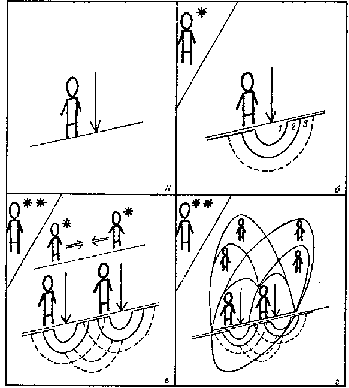
\includegraphics[width=.5\textwidth]{activity-nature-system.png}
\end{center}

Es ist davon auszugehen, dass der Kern der ökologischen Situation durch den
Fakt des Zusammentreffen mehrerer unterschiedlicher Handlungssysteme innerhalb
eines Naturraums oder einer Fläche natürlichen Materials gegebn ist. Der
Ausgangspunkt für die Analyse der ökologischen Situation ist die
Handlungsstruktur, die bewusst gerichtet oder nicht zielgerichtet auf die
Natur wirkt. Im Diagramm kann eine solche Handlungsstruktur bedingt durch das
Zeichen \emph{„Position“} und das Zeichen „Einwirkung“ auf das natürliche
Material gekennzeichnet werden (siehe Abbildung). Jede Position ist durch ihre
spezifischen Werte, Ziele, Setzungen, Mittel, Methoden sowie Denk- und
Handlungsweisen gekennzeichnet. Die Position kann nicht auf einen bloßen
Unterschied der Mittel reduziert werden, obwohl jede Position durch eine
bestimmte Vorstellung vom Objekts charakterisiert werden kann und folglich
durch eine bestimmte Kombination von Handlungsmitteln. Allerdings können
einzelne Mittel von einer Position zur anderen wechseln und wechseln auch.

Eine Position ist also durch eine besondere Schnittmenge vieler Beziehungen
gegeben: vor allen durch ihre Orientierung auf eine bestimmte Art von Praxis
und folglich durch die möglichen Weisen der Nutzung von Wissen. Das Prinzip
der Gerichtetheit des Wissens auf diese oder jene Art von Tätigkeit und die
eigentümliche Unterordnung des Wissens unter die Praxis dieser oder jener Art
von Praxis erlaubt es, die Handlungsstrukturen mit Hilfe von grafischen
Symbolzeichen -- „Positionen“ -- darzustellen.

Allerdings wird allein durch die Tatsache der Einwirkung auf das natürliche
Material durch diese oder jene Handlungsquelle noch keine ökologische
Situation geschaffen. Ein notwendiges Element der Situation ist eine reflexive
Position, die Position des externen Beobachters -- dargestellt als „Position
mit Sternchen“ (siehe Abb. 1b). Genau in dieser Position eines „äußeren“
Beobachters und Analytiker, werden die Folgen der Einwirkung auf das
natürliche Material fixiert. Die erste Aufstellung des ökologischen Problems
hat damit zu tun, dass der externe Beobachter beginnt, im Namen der Natur zu
sprechen; er hebt die Folgen einzelner Wirkungen auf die Umwelt hervor und
macht sie zum zentralen Moment der Analyse der faktischen Diskrepanz und
Divergenz zwischen den Zielen der künstlich-technische Handlungen und den
Ergebnissen der realen Auswirkungen auf die Natur.

Auch wenn sich in der Geschichte der Bildung und Formierung des ökologischen
Standpunktes reale Beobachter -- von Marsh und der Chicagoer Schule der
Stadtökologie bis zu den Autoren des Club of Rome -- nur allmählich von einer
unmittelbaren und phänomenalen Sicht auf lokale Auswirkungen anthropogener
Einflüsse zu einer Analyse der tieferen und langfristigen Folgen der
wissenschaftlich-technischen Revolution als Ganzes bewegten, so werden wir
doch im Schema der einfachsten ökologischen Situation mindestens drei „Zonen“
von Folgen fixieren. Die erste Zone betrifft die beherrschbaren und
zurechenbaren Folgen, die zweite die unbeherrschbaren, aber zurechenbaren
Folgen und die dritte Zone die unbeherrschbaren und nicht zurechenbaren
Folgen.  Die Merkmale \emph{„Beherrschbarkeit“} und \emph{„Zurechenbarkeit“}
beziehen sich jeweils auf die Handlung selbst und ihre reflexive Begleitung.

Die eingeführte Schematisierung hat großen Sinn im Plan der Kritik an den
bestehenden Ansätzen: Aus ihr folgt u.a., dass alle die Schulen und
Richtungen, die nur mit zurechenbaren, vorhersehbaren Konsequenzen arbeiten,
die Struktur der ökologischen Situation bewusst unrichtig darstellen und auf
übervereinfachten Schemata von Objekten arbeiten. Die hervorgehobenen „Zonen“
fixieren eine funktionale Struktur des Raums der Folgen, und in diesem Plan
erweisen sich unbeherrschbare und nicht zurechenbare Folgen als grundsätzlich
„zugerechnet“ auf Kosten der Verwendung dieser Art von Abbild-Schema der
ökologischen Situation.

Die Struktur der ökologischen Situation wäre jedoch grundsätzlich
unvollständig, wenn wir auf die eingeführten Vorstellungrn beschränken
würden. Das konstitutive Moment der Situation ist das „Erscheinen“ einer
anderen Handlungsstruktur, die im selben Naturareal lokalisiert ist. In diesem
Fall müssen die „Folgen“ der ersten Einwirkung als „Bedingungen“ für die
Entfaltung des anderen Handelns betrachtet werden. Wenn es auf demselben
natürlichen Material mehrere verschiedene Arten und Formen von Handeln gibt,
dann ändert sich das Bild der Folgen grundlegend. Die Folgen, die vom neuen
Handlungssystem verursacht werden, „überlagern“ die anfänglichen funktionale
Struktur der Folgen überlagert (siehe Abb. 1c), es entsteht eine „Interferenz“
und die Grenzen der „Zone“ der bilanzierte und nicht bilanzierte Folgen
verschiebt und ändert sich. Es entsteht und verbreitert sich eine Kette von
„sekundären“ ökologischen Effekten.

Wenn sich zwei oder mehr verschiedene Handlungsstrukturen auf demselben
natürlichen Material entwickeln, sollten neben Folgen der Einwirkung auf das
Naturmaterial auch berücksich\-tigt und analysiert werden
\begin{enumerate}
\item der Einfluss einer Handlungsstruktur auf andere Strukturen durch den
  unmittelbarn Handlungskontext;
\item Folgen der Einwirkung auf andere Handlungsstrukturen durch das
  „eroberte“ und modifizierte Naturmaterial (das in diesem Fall als
  Übertragungsglied wirkt);
\item Folgen der Einwirkung auf das Naturmaterial durch Veränderungen und
  Transformation von „benachbarten“ Handlungsstrukturen. 
\end{enumerate}
Dabei verschiebt sich das Zentrum der ökologischen Situation naturgemäß von
einem „Hand\-lungs-Natur“-Verhältnis zu einem Verhältnis von „Aktivität 1 zu
Aktivität 2“; es entstehen eine Reihe von neuen Konflikten und Widersprüchen
zwischen den Strukturen und Handlungssystemen, die auf ein und demselben
Naturmaterial „parasitieren“.

Wenn wir es in den ersten Schritten der Entfaltung der ökologischen Situation
mit Folgen als „Antwortschlag“ der Natur zu tun hatten, so haben wir es jetzt
mit Folgen zu tun, die durch das Primsa der „Sicht“ reflektiert und gebrochen
sind, durch die Handlungsinteressen anderer Akteure in der Situation, durch
andere Positionen und andere Arten von Handlungen. „Saurer Regen“ fällt auf
das Gebiet eines benachbarten Staates, und es entsteht ein internationaler
Konflikt. Die Emissionen eines Gas fördernden Komplexes schädigen
Reisanpflanzungen, und es entwickelt sich ein Zusammenstoß zwischen zwei
Ministerien. Die Luftverschmutzung verursacht eine Zunahme von
Lungenkrankheiten, und das Gesundheitsministerium verklagt die
Industrieverbände der Stadt. Dabei ist es sehr schwierig, eine Grenze zu
ziehen zwischen einer Situation, in der verschiedene Handlungstypen
miteinander interagieren, und einer Situation der Einwirkung auf die
natürliche Umwelt.  Der ganze Komplex von Ungereimtheiten und Widersprüchen in
der Organisation und Ko-Organisation von Handeln ist wie „hineingezogen“ in
die ökologische Situation und verändert kardinal deren Konturen.

Die wichtigsten Komponenten der ökologischen Situation sind die folgenden: die
Organisa\-tions- und Managementstrukturen (siehe Abb. 1d), \emph{Konflikte}
zwischen verschiedenen Handlungsstrukturen und deren steuerndem „Überbau“
bezüglich der bevorzugten Formen der Nutzung und Verwendung des natürlichen
Materials.  Jede Handlungsstruktur ist ständig damit konfrontiert, dass auf
das eigene System der Verwendung von Naturmaterial andere Handlungen
einwirken.  „Was machen Sie mit der Natur?“ -- fragt man die einen. Aber das
ist jedesmal anders zu verstehen: „Warum lässt du mich die Natur nicht auf
eine viel „progressivere“ Art nutzen und schädigen?“. Und in diesem Chor der
Stimmen, der in der heutigen ökologischen Situation erklingt, mischen und
verflechten sich die Stimmen der außenstehenden Beobachter, die im Namen der
Natur sprechen, mit den Stimmen derer, die im Namen des Handelns sprechen --
interessiert, eigene spezifische, insbesondere bereichsgebundene Ziele und
Aufgaben verfolgend. Und dabei müssen diejenigen, die sich heute das Recht
anmaßen, für die Natur im Namen „höchster Werte“ zu sprechen, sich ebenfalls
einer besonderen und sorgfältigen „Prüfung“ unterziehen, auf welche Art von
Werten und Zielen sie sich dabei orientieren, und auf welche Art von Praxis
es als Ergebnis der Entfaltung dieser Werte und Ziele hinausläuft.

So wird die Struktur der ökologischen Situation immer komplexer. Wir fixieren
im Schema Fixierung nur die Positionssymbole, und überlassen es dem Leser, die
realen Widersprüche und Konflikte zu rekonstruieren und zu Ende zu denken,
deren Zeuge er heute ist. Gleichzeitig lassen wir ihm die Freiheit, dieses
„Positionsspiel“ fortzusetzen: man kann in die gegebene schematische
Darstellung sukzessive neue Positionen einführen, wodurch das Schema immer
komplexer wird und weitere Schichten der realen Situation erfasst werden. An
dieser Stelle können alarmistische Wissenschaftler ins Spiel kommen, die sich
auf konkrete Erscheinungsformen der Folgen orientiert haben -- Verschmutzung
der Luft, des Wassers, Krise der städtischen Umwelt; es werden Vertreter von
alternativen Umweltbewegungen mit ihren politischen Interessen erscheinen, die
dazu zwingen, unter Ausnutzung sekundärer ökologischer Effekte, ihnen neuen
Klang zu geben und de Status eines globalen Problems; hier sind Vertreter
verschiedener organisatorisch-steuernder Überbauten einzuschließen --
beginnend mit Ministerien und Behörden mit ihren spezifischen Interessen und
entwickelten Beziehungen zur Situation „vor Ort“, und endend mit Gremien der
territorialen und regionalen Steuerung, welche die ökologische Situation
nutzen, um eine Poltik der Dezentralisierung durchzusetzen und Einfluss auf
die Strukturen der sektoralen Führung zu gewinnen.

Zugleich demonstriert die durchgeführte Analyse anschaulich, dass die
ökologische Situation vor allem eine soziale und Handlungssituation ist. Ohne
diejenigen Aspekte der Situation zu rekonstruieren, bei denen ökologische
Fragen und Folgen zu einem Mittel des politischen Kampfes und der Steuerung
werden, des organisatorischen Einflusses und der direkten Nötigung, wo sich
Zusammenstöße und Konflikte zwischen verschiedenen Handlungstypen entfalten,
kann man das Wesen und die Substanz der ökologischen Situation nicht
verstehen.  Dies ist gut und detaillierter am Beispiel der urbanistischen
Situation in der Arbeit von E. Epishin „Program 'ecopolis'“\footnote{
  \foreignlanguage{russian}{Е. Епишин «Программа 'экополис'» (ЧиП, 1986, №
    9)}} dargestellt. Ohne die heute existierenden Tendenzen in der
Organisation und Verwaltung verschiedener Handlungssysteme zu sehen, die auf
ein und demselben natürlichen Material parasitieren, ist es unmöglich, die
Struktur und die Grenzen von Ökosystemen zu bestimmen. Man kann auh nicht
umhin, den Fakt zu berücksichtigen, dass die einen Managementstrukturen nur
darauf ausgerichtet sind, verschiedene Handlungsarten zu koordinieren, während
andere im Gegensatz dazu das natürliche Material und die abgeteilten Zonen der
Folgen selbst als Objekt in ihr Managements einbeziehen.  

In einem Fall werden wir es mit einer Kompromissökologie zu tun haben. Im
anderen sind wir gezwungen, die Möglichkeiten und zulässigen Arten der
Verwendung des natürlichen Materials zu analysieren; wenn wir die Organisation
des Handelns betrachten, müssen wir uns folgende Fragen stellen: welche Formen
der Nutzung des Naturraumes schließen wir, indem wir diese oder jene
strategische Entscheidung treffen, welche Formen der Nutzung werden unmöglich?
Ausgehend von den Begriffen Ressource, Territorium, Bedingungen entwickeln wir
ein alternatives Design und eine Projektion solcher Technologien und
Handlungssysteme, die es heute noch nicht gibt.  Dann wird das „Natürliche“,
die Analyse der Folgen und der ökologischen Situation nur ein Moment einer
\emph{alternativen projektierenden Arbeit}, und führt gleichzeitig zur
\emph{Programmierung der Entwicklung} des HNS.

\begin{center}
  * * *
\end{center}

Damit haben wir ein einfachstes Schema der ökologischen Situation eingeführt
und Wege seiner Entfaltung skizziert. Bedeutet dies, dass wir die Struktur des
HNS gegeben haben? Nein. Bis jetzt ist nur das objekt-ontologische Feld
gegeben, der „Hintergrund“, vor dem Handlungs-Natur-Systeme verschiedener
Komplexitätsstufen „skizziert“ und „ausgeschnitten“ werden können.  Die
Grenzen der verschiedenen HNS werden dadurch definiert, welchen praktischen
Rahmen wir annehmen und unter welchem „Blickwinkel“ der zentrale,
systembildende Faktor und der grundlegende Prozess abgehoben wird, der die
Ganzheit des gegebenen HNS ausmacht.

Wenn wir anfangen, über HNS zu sprechen, versichern uns Forscher und Planer,
dass ein HNS aus zwei Teilsystemen besteht: dem Handlungs- und dem
Natursystem.  So reproduzieren sie durch die Anwendung von strukturellen
Analysemethoden den methodologischen Dualismus und führen eine Reihe von
schwerfälligen und aufgrund der akzeptierten Formulierung unlösbaren Problemen
ein. Im 19. Jahrhundert führte die gleiche Art naiver Metaphysik zur
Entstehung und weiten Verbreitung des Problems des Verhältnisses von „Geist“
und „Körper“. Heute verstehen wir, dass, solange wir die technische Arbeit mit
dem Menschen in die Praxis der Arbeit mit seiner Physiologie und die Praxis
der Arbeit mit seiner Psychologie teilen, psychophysikalische und
psychophysiologische Problemen existieren werden. Es lohnt nicht, die
logischen und methodologischen Fehler, die von den Psychologen des letzten
Jahrhunderts gemacht wurden, im Bereich der Ökonomie zu wiederholen.  Indem
wir Anleihen an einer naiven „Metaphysik der Natur“ nehmen und diese einem
„technischen“ Teilsystem der Natur gegenüberstellen, erzeugen wir eine Reihe
von Pseudoproblemen und falschen Lösungen und verschließen uns im Kern die
Möglichkeit des Übergangs zu einer realen Projektierung und Erforschung des
HNS.

Das HNS ist ein einheitliches System und kann nicht in zwei oder mehrere
Teilsysteme „zerschnitten“ werden. Im Kern behauptet die Ideologie des
Systemansatzes auch, dass das betreffende Objekt nicht in Teile und Subsysteme
aufgeteilt werden kann, sondern als eins, als Einheit genonnen werden muss.

Die eingeführte schematische Darstellung der ökologischen Situation fokussiert
auf den Fakt, dass die Handlungsstrukturen das Naturmaterial „ergreifen“, es
auf besondere Weise transformieren und umarbeiten, es teilweise assimilieren
und teilweise transformieren in Übereinstim\-mung mit dem Charakter der
anthropogenen und technogenen Aktivitäten.

Allerdings ist Zugriff auf die Arten von Material, die der Form nicht
entsprechen, ihr real-praktisch entgegenstehen, im Kern der erste Schritt zu
einer völlig anderen, nicht-materiellen Behandlung des Naturmaterials. Das
Material erscheint in dieser Wendung selbst als \emph{vollstän\-diges System},
das nach seinen eigenen Gesetzen lebt und seine eigenen spezifischen Prozesse
hat. Mit anderen Worten, nicht die Form steht dem Material entgegen, sondern
die Prozesse, welche das gesamte handelnde, technische System konstituieren,
stehen anderen Prozessen gegenüber, die ein anderes vollständiges System
konstituieren.  Anstelle der recht einfachen und naheliegenden Kategorie
„Form-Material“ sind wir gezwungen uns viel komplexeren Kategorien des
Systemansatzes zuzuwenden.  Ein „System-Zentaur“ ist im methodologischen Plan
ein \emph{Polysystem}, in dessen Rahmen die einen Prozesse und Systeme zum
Material werden, auf dem sich andere Prozesse und für diese spezifische
funktionale Strukturen entfalten.

Der Schwerpunkt der systemischen Analyse verlagert sich zur Identifizierung
verschiedener Möglichkeiten der „Aufreihung“ von Handlungs- und
Naturprozessen, von natürlich-geschichtlichen Prozessen, zur Analyse der
Mechanismen der „Verkünstlichung“ natürlicher und „Naturalisierung“
technischer Komponenten, auf die Durcharbeitung der zusätzlichen Kategorien
Bedingungen, Folgeen, Ressource, Grenzen und anderer.

Indem auf den umlaufenden Begriff der Natur verzichtet und die Setzung eines
neuen Konzept der „zweiten Natur“ und eines neuen „Konzepts der Rationalität“
angenommen wird, das auf „System-Zentauren“ angewendet werden kann, müssen wir
gesetzmäßig die Frage einer praktischen und logisch-methodologische Wende im
weiteren Sinne stellen. Es ist notwendig, andere, komplexere systemische
Kategorien heranzuziehen und nicht nur und nicht so sehr die kategorialen
Gegensätze „Teil -- Ganzes“, „Element -- Verbindung“ und „Form -- Material“ zu
betrachten als vielmehr Beziehungen „Prozess -- Material“, „Funktion --
Morphologie“, „Prozess -- Struktur“, Beziehungen und Korrelationen zwischen
den prozessualen, strukturell-funktionalen, morphologischen und „materiellen“
Vorstellungen komplexer Systeme. Die Aufgaben der Anwendung der systemischen
Methodologie bei der Analyse ökologischer Situationen demonstriert anschaulich
das Defizit vorhandener Vorstellungen; die Setzungen im ontologischen Bild der
techno-natürlichen Welt stellen neue Aufgaben vor den Systemansatz.

Um zur Abhebung eines „kompletten“ HNS überzugehen, ist es jetzt notwendig,
von der Position eines externen \emph{Beobachters überzugehen in die Position
  der Organisation und Handlung} in Bezug auf die gesamte Konfiguration
verschiedener Aktivitäten mit natürlichen Material. Ohne eine Position des
Handelns in Bezug auf die ökologische Situation einzunehmen, kann man über die
ökologische Situation sprechen, aber keine HNS projektieren und erforschen. Im
Gegenteil, durch die Einnahme der einen oder anderen \emph{praktischen
  organisatorischen Position} kann man den einen oder anderen grundlegenden
„Basis“-Prozess herausheben und und die ihm entsprechenden funktionale
Strukturen und Grenzen des HNS. Das „Ausschneiden“ vollständiger Systeme in
der Theorie ist in einem rein abstrakten Sinn nicht möglich; nur durch die
Erstellung eines HNS und Hervorhebung von dessen „arbeitenden“
Managementprinzipien kann man die ökologische Situationen lösen.

Und die Ökologie akkumuliert in dieser neuen Wendung in sich die
\emph{praktischen Motive der der gegenwärtigen Situation} und sorgt für die
Transformation der Technik und der Poesie des Fortschritts in die Praxis der
Konstruktion des Lebens und die Entwicklung der Lebenstätigkeit und des
Handelns der Menschen.

In dieser Richtung haben wir nur die ersten Schritte gemacht, auf jedem
stießen wir auf Mythen und Gespenster des wissenschaftlichen und alltäglichen
Bewusstseins, auf die Idole des „Platzes“ und die Idole des „Marktes“, auf
deren Bedeutung schon F. Baacon hingewiesen hat. Es kann sein, dass es uns
gelingt, inmitten der Vielfalt und Buntheit der Standpunkte, im Chaos der
Meinungen und Programme, jenen Weg zu erfühle, den die Ökologie des neuen
Jahrhunderts gehen kann und muss.

\section{Bibliographie}

\foreignlanguage{russian}{
\begin{enumerate}
\item Андерсен Дж. М. Экология и науки об окружающей среде: биосфера,
  экосистемы, человек. — М., «Мысль», 1985.
\item Анучин В. А. Основы природопользования. Теоретический аспект. — М.,
  «Наука», 1987.
\item Глазычев В. Л. Социально-экологическая интерпретация городской среды. —
  М., «Наука», 1984.
\item Епишин В. К. Три методологических подхода в современной геологии.
  Системо-мыследеятельностный подход: понятие «геосистемы». // В сборнике:
  Системно-геологические исследования литосферы. — М., 1985.
\item Епишин В. К., Епишин Е. В. Геология как сфера деятельности
  (системно-аксио\-логический подход). // В сборнике: Системные исследования и
  разработки в геологии. — М., МОИП, 1985.
\item Епишин Е. В. Программа «экополис». — Человек и природа. — 1986. — № 9.
\item Епишин Е. В. Авариеведение. — Человек и природа. — 1987. — № 8.
\item Ойзерман М. Т., Рац М. В., Щедровицкий Г. П. Научные и практические
  вопросы создания эффективно реализуемых проектов с точки зрения изысканий.
  // В сборнике: Прометодологии и технологии инженерных изысканий. — М., 1985.
\item Сен-Марк Ф. Социализация природы. — М., «Прогресс», 1977.
\item Фёдоров В. Д., Гильмаиов Т. Б. Экология. — М., МГУ, 1980.
\item Щедровицкий Г. П. Проблемы методологии системного исследования. — М.,
  Знание, 1964.
\item Щедровицкий Г. П. Принципы и общая схема методологической организации
  сис\-темно-структурных исследовании и разработок. // Ежегодник «Системные
  исследования». — М., «Наука», 1981.
\end{enumerate}
}

\end{document}
